\documentclass[11pt,a4paper,oneside]{report}             % Single-side
%\documentclass[11pt,a4paper,twoside,openright]{report}  % Duplex

%\PassOptionsToPackage{chapternumber=Huordinal}{magyar.ldf}
\usepackage{t1enc}
\usepackage[latin2]{inputenc}
\usepackage{amsmath}
\usepackage{amssymb}
\usepackage{enumerate}
\usepackage[thmmarks]{ntheorem}
\usepackage{graphics}
\usepackage{epsfig}
\usepackage{listings}
\usepackage{color}
%\usepackage{fancyhdr}
\usepackage{lastpage}
\usepackage{anysize}
%\usepackage[magyar]{babel}
\usepackage{sectsty}
\usepackage{setspace}  % Ettol a tablazatok, abrak, labjegyzetek maradnak 1-es sorkozzel!
\usepackage[hang]{caption}
\usepackage{hyperref}
\usepackage{amsmath}
\usepackage{tcolorbox}
\usepackage{longtable}
\usepackage{algorithm2e}
\usepackage{multirow}

\usepackage{titlesec}
\tcbuselibrary{listings,breakable}

%--------------------------------------------------------------------------------------
% Main variables
%--------------------------------------------------------------------------------------
\newcommand{\vikszerzo}{G�mes Kinga Andrea}
\newcommand{\vikkonzulens}{Kov�cs �d�m}
\newcommand{\vikcim}{Deep learning of graph transformations}
\newcommand{\viktanszek}{Department of Automation and Applied Informatics}
\newcommand{\vikdoktipus}{Masters Thesis}
\newcommand{\vikdepartmentr}{G�mes Kinga Andrea}
\newcommand{\textbox}[2]{\begin{tcolorbox}[breakable,
		title after break=,
		left=0mm,right=0mm,bottom=0mm,top=0mm,
		%enforce breakable,% <-- never use this
		%break at=8cm,
		pad at break=1mm,
		]{#1}
\end{tcolorbox}}

%--------------------------------------------------------------------------------------
% Page layout setup
%--------------------------------------------------------------------------------------
% we need to redefine the pagestyle plain
% another possibility is to use the body of this command without \fancypagestyle
% and use \pagestyle{fancy} but in that case the special pages
% (like the ToC, the References, and the Chapter pages)remain in plane style

\pagestyle{plain}
%\setlength{\parindent}{0pt} % �ttekinthet�bb, angol nyelv� dokumentumokban jellemz�
%\setlength{\parskip}{8pt plus 3pt minus 3pt} % �ttekinthet�bb, angol nyelv� dokumentumokban jellemz�
\setlength{\parindent}{12pt} % magyar nyelv� dokumentumokban jellemz�
\setlength{\parskip}{0pt}    % magyar nyelv� dokumentumokban jellemz�

\marginsize{35mm}{25mm}{15mm}{15mm} % anysize package
\setcounter{secnumdepth}{0}
\sectionfont{\large\upshape\bfseries}
\setcounter{secnumdepth}{5}
\singlespacing
\frenchspacing


\titleformat{\paragraph} {\normalfont\normalsize\bfseries}{\theparagraph}{1em}{}
\titlespacing*{\paragraph} {0pt}{3.25ex plus 1ex minus .2ex}{1.5ex plus .2ex}

%--------------------------------------------------------------------------------------
%	Setup hyperref package
%--------------------------------------------------------------------------------------
\hypersetup{
    bookmarks=true,            % show bookmarks bar?
    unicode=false,             % non-Latin characters in Acrobat�s bookmarks
    pdftitle={\vikcim},        % title
    pdfauthor={\vikszerzo},    % author
    pdfsubject={\vikdoktipus}, % subject of the document
    pdfcreator={\vikszerzo},   % creator of the document
    pdfproducer={Producer},    % producer of the document
    pdfkeywords={keywords},    % list of keywords
    pdfnewwindow=true,         % links in new window
    colorlinks=true,           % false: boxed links; true: colored links
    linkcolor=black,           % color of internal links
    citecolor=black,           % color of links to bibliography
    filecolor=black,           % color of file links
    urlcolor=black             % color of external links
}

%--------------------------------------------------------------------------------------
% Set up listings
%--------------------------------------------------------------------------------------
\lstset{
	basicstyle=\scriptsize\ttfamily, % print whole listing small
	keywordstyle=\color{black}\bfseries\underbar, % underlined bold black keywords
	identifierstyle=, 					% nothing happens
	commentstyle=\color{white}, % white comments
	stringstyle=\scriptsize\sffamily, 			% typewriter type for strings
	showstringspaces=false,     % no special string spaces
	aboveskip=3pt,
	belowskip=3pt,
	columns=fixed,
	backgroundcolor=\color{lightgray},
} 		
\def\lstlistingname{lista}	

%--------------------------------------------------------------------------------------
%	Some new commands and declarations
%--------------------------------------------------------------------------------------
\newcommand{\code}[1]{{\upshape\ttfamily\scriptsize\indent #1}}

% define references
\newcommand{\figref}[1]{\ref{fig:#1}.}
\renewcommand{\eqref}[1]{(\ref{eq:#1})}
\newcommand{\listref}[1]{\ref{listing:#1}.}
\newcommand{\sectref}[1]{\ref{sect:#1}}
\newcommand{\tabref}[1]{\ref{tab:#1}.}

\DeclareMathOperator*{\argmax}{arg\,max}
%\DeclareMathOperator*[1]{\floor}{arg\,max}
\DeclareMathOperator{\sign}{sgn}
\DeclareMathOperator{\rot}{rot}
\definecolor{lightgray}{rgb}{0.95,0.95,0.95}

\author{\vikszerzo}
\title{\viktitle}
\includeonly{
	project,%
	titlepage,%
	declaration,%
	abstract,%
	introduction,%
	chapter0,
	chapter1,%
	chapter2,%
	chapter3,%
	chapter4,%
	chapter5,%
	acknowledgement,%
	appendices,%
}
%--------------------------------------------------------------------------------------
%	Setup captions
%--------------------------------------------------------------------------------------
\captionsetup[figure]{
%labelsep=none,
%font={footnotesize,it},
%justification=justified,
width=.75\textwidth,
aboveskip=10pt}

\renewcommand{\captionlabelfont}{\small\bf}
\renewcommand{\captionfont}{\footnotesize\it}

%--------------------------------------------------------------------------------------
% Table of contents and the main text
%--------------------------------------------------------------------------------------
\begin{document}
\singlespacing
%%--------------------------------------------------------------------------------------
% Rovid formai es tartalmi tajekoztato
%--------------------------------------------------------------------------------------

\footnotesize
\begin{center}
\large
\textbf{\Large �ltal�nos inform�ci�k, a diplomaterv szerkezete}\\
\end{center}

A diplomaterv szerkezete a BME Villamosm�rn�ki �s Informatikai Kar�n:
\begin{enumerate}
\item	Diplomaterv feladatki�r�s
\item	C�moldal
\item	Tartalomjegyz�k
\item	A diplomatervez� nyilatkozata az �n�ll� munk�r�l �s az elektronikus adatok kezel�s�r�l
\item	Tartalmi �sszefoglal� magyarul �s angolul
\item	Bevezet�s: a feladat �rtelmez�se, a tervez�s c�lja, a feladat indokolts�ga, a diplomaterv fel�p�t�s�nek r�vid �sszefoglal�sa
\item	A feladatki�r�s pontos�t�sa �s r�szletes elemz�se
\item	El�zm�nyek (irodalomkutat�s, hasonl� alkot�sok), az ezekb�l levonhat� k�vetkeztet�sek
\item	A tervez�s r�szletes le�r�sa, a d�nt�si lehet�s�gek �rt�kel�se �s a v�lasztott megold�sok indokl�sa
\item	A megtervezett m�szaki alkot�s �rt�kel�se, kritikai elemz�se, tov�bbfejleszt�si lehet�s�gek
\item	Esetleges k�sz�netnyilv�n�t�sok
\item	R�szletes �s pontos irodalomjegyz�k
\item	F�ggel�k(ek)
\end{enumerate}

Felhaszn�lhat� a k�vetkez� oldalt�l kezd�d� \LaTeX-Diplomaterv sablon dokumentum tartalma. 

A diplomaterv szabv�nyos m�ret� A4-es lapokra ker�lj�n. Az oldalak t�k�rmarg�val k�sz�ljenek (mindenhol 2.5cm, baloldalon 1cm-es k�t�ssel). Az alap�rtelmezett bet�k�szlet a 12 pontos Times New Roman, m�sfeles sork�zzel.

Minden oldalon - az els� n�gy szerkezeti elem kiv�tel�vel - szerepelnie kell az oldalsz�mnak.

A fejezeteket decim�lis beoszt�ssal kell ell�tni. Az �br�kat a megfelel� helyre be kell illeszteni, fejezetenk�nt decim�lis sz�mmal �s kifejez� c�mmel kell ell�tni. A fejezeteket decim�lis al�oszt�ssal sz�mozzuk, maxim�lisan 3 al�oszt�s m�lys�gben (pl. 2.3.4.1.). Az �br�kat, t�bl�zatokat �s k�pleteket c�lszer� fejezetenk�nt k�l�n sz�mozni (pl. 2.4. �bra, 4.2 t�bl�zat vagy k�pletn�l (3.2)). A fejezetc�meket igaz�tsuk balra, a norm�l sz�vegn�l viszont haszn�ljunk sorkiegyenl�t�st. Az �br�kat, t�bl�zatokat �s a hozz�juk tartoz� c�met igaz�tsuk k�z�pre. A c�m a jel�lt r�sz alatt helyezkedjen el.

A k�peket lehet�leg rajzol� programmal k�sz�ts�k el, az egyenleteket egyenlet-szerkeszt� seg�ts�g�vel �rj�k le (A \LaTeX~ehhez k�zenfekv� megold�sokat ny�jt).

Az irodalomjegyz�k sz�vegk�zi hivatkoz�sa t�rt�nhet a Harvard-rendszerben (a szerz� �s az �vsz�m megad�s�val) vagy sorsz�mozva. A teljes lista n�vsor szerinti sorrendben a sz�veg v�g�n szerepeljen (sorsz�mozott irodalmi hivatkoz�sok eset�n hivatkoz�si sorrendben). A szakirodalmi forr�sok c�meit azonban mindig az eredeti nyelven kell megadni, esetleg z�r�jelben a ford�t�ssal. A list�ban szerepl� valamennyi publik�ci�ra hivatkozni kell a sz�vegben (a \LaTeX-sablon a Bib\TeX~seg�ts�g�vel mindezt automatikusan kezeli). Minden publik�ci� a szerz�k ut�n a k�vetkez� adatok szerepelnek: foly�irat cikkekn�l a pontos c�m, a foly�irat c�me, �vfolyam, sz�m, oldalsz�m t�l-ig. A foly�irat c�meket csak akkor r�vid�ts�k, ha azok nagyon k�zismertek vagy nagyon hossz�ak. Internet hivatkoz�sok megad�sakor fontos, hogy az el�r�si �t el�tt megadjuk az oldal tulajdonos�t �s tartalm�t (mivel a link egy id� ut�n ak�r el�rhetetlenn� is v�lhat), valamint az el�r�s id�pontj�t.

\vspace{5mm}
Fontos:
\begin{itemize}
	\item A szakdolgozat k�sz�t� / diplomatervez� nyilatkozata (a jelen sablonban szerepl� sz�vegtartalommal) k�telez� el��r�s Karunkon ennek hi�ny�ban a szakdolgozat/diplomaterv nem b�r�lhat� �s nem v�dhet� !
	\item Mind a dolgozat, mind a mell�klet maxim�lisan 15 MB m�ret� lehet !
\end{itemize}

\vspace{5mm}
\begin{center}
J� munk�t, sikeres szakdolgozat k�sz�t�st ill. diplomatervez�st k�v�nunk !
\end{center}

\normalsize

%--------------------------------------------------------------------------------------
% Feladatkiiras (a tanszeken atveheto, kinyomtatott valtozat)
%--------------------------------------------------------------------------------------
\clearpage
\begin{center}
\large
\textbf{FELADATKI�R�S}\\
\end{center}

A szemantikai elemz�s c�lja, hogy term�szetes nyelvi adathoz k�sz�thess�nk szemantikai reprezent�ci�t, �gy tudjuk modellezni a sz�veg jelent�s�t. Ha a nyelvi jelent�st fogalmak ir�ny�tott gr�fjaival reprezent�ljuk, ezeket pedig a mondat szintaktikai szerkezet�t reprezent�l� f�kb�l kell el\H{o}�ll�tanunk, akkor a teljes feladat egyetlen komplex gr�ftranszform�ci�k�nt defini�lhat�.
A n�pszer\H{u} szemantikai feladatokra, mint a szemantikai hasonl�s�g m�r�se vagy a g�pi sz�veg�rt�s, ritk�n haszn�lj�k a term�szetes nyelv szemantik�j�nak gr�fos reprezent�ci�j�t,
f\H{o}leg state-of-the art rendszerekben. Ezek a rendszerek t�bbnyire sz� embeddingeket haszn�lnak szavak jelent�s�nek �br�zol�s�ra, amik a szavak jelent�s�t legfeljebb neh�ny sz�z dimenzi�s val�s vektork�nt �br�zolj�k.
Egy �j k�s�rleti megk�zel�t�s a gr�f-transzform�ci�k k�zvetlen tanul�sa, amely sor�n gr�f-h�l�zatokat haszn�lva ezek a szemantikai reprezent�ci�k gr�f form�ban val� transzform�l�sa is lehets�ges lenne. 

Ilyen feladatot t�mogat� keretrendszerek p�ld�ul a Graph Nets Library (ld. \href{https://github.com/deepmind/graph\_nets}{GitHub})
vagy a Deep Graph Library (ld. \href{https://github.com/dmlc/dgl}{GitHub}). A hallgat� munk�j�nak k�zponti t�m�j�t az erre ir�nyul�
k�s�rletek adj�k. A hallgat� feladatai a k�vetkez\H{o}kre terjednek ki:
\begin{itemize}
\item Ismerjen meg egy gr�f-h�l�zatok tanul�s�ra ir�nyul� keretrendszert.
\item V�gezzen k�s�rleteket gr�f-transzform�ci�k m�ly tanul�s�ra.
\item Ismerjen meg legal�bb egy szemantikai reprezent�ci�t ig�nyl\H{o} feladatot, ahol a m�dszer k�zvetlen �rt�kelhet\H{o} lenne, p�ld�ul a Surface Realization
(ld. \href{http://taln.upf.edu/pages/msr2018-ws/SRST.html}{Surface Realization cikk}) vagy az Extractive Summarization.
\item V�gezzen k�zvetlen k�s�rleteket a szemantikai reprezent�ci�t ig�nyl\H{o} feladaton.
\item M�rje fel a rendszer korl�tait az eredm�nyek ki�rt�kel�s�n kereszt�l.
\end{itemize}





\pagenumbering{arabic}
\onehalfspacing
%--------------------------------------------------------------------------------------
%	The title page
%--------------------------------------------------------------------------------------
\begin{titlepage}
\begin{center}

\includegraphics[width=60mm,keepaspectratio]{figures/BMElogo.png}\\
\vspace{0.3cm}
\textbf{Budapest University of Technology and Economics}\\
\textmd{Faculty of Electrical Engineering and Informatics}\\
\textmd{\viktanszek}\\[5cm]

\vspace{0.4cm}
{\huge \bfseries \vikcim}\\[0.8cm]
\vspace{0.5cm}
\textsc{\Large \vikdoktipus}\\[4cm]

\begin{tabular}{cc}
 \makebox[7cm]{\emph{Written By}} & \makebox[7cm]{\emph{Consultant}} \\
 \makebox[7cm]{\vikszerzo} & \makebox[7cm]{\vikkonzulens}
\end{tabular}

\vfill
{\large \today}
\end{center}
\end{titlepage}



\tableofcontents\vfill
%--------------------------------------------------------------------------------------
% Nyilatkozat
%--------------------------------------------------------------------------------------
\begin{center}
\large
\textbf{HALLGAT�I NYILATKOZAT}\\
\end{center}

Alul�rott \emph{\vikszerzo}, szigorl� hallgat� kijelentem, hogy ezt a diplomatervet meg nem engedett seg�ts�g n�lk�l, saj�t magam k�sz�tettem, csak a megadott forr�sokat (szakirodalom, eszk�z�k stb.) haszn�ltam fel. Minden olyan r�szt, melyet sz� szerint, vagy azonos �rtelemben, de �tfogalmazva m�s forr�sb�l �tvettem, egy�rtelm�en, a forr�s megad�s�val megjel�ltem.

Hozz�j�rulok, hogy a jelen munk�m alapadatait (szerz�(k), c�m, angol �s magyar nyelv� tartalmi kivonat, k�sz�t�s �ve, konzulens(ek) neve) a BME VIK nyilv�nosan hozz�f�rhet� elektronikus form�ban, a munka teljes sz�veg�t pedig az egyetem bels� h�l�zat�n kereszt�l (vagy autentik�lt felhaszn�l�k sz�m�ra) k�zz�tegye. Kijelentem, hogy a beny�jtott munka �s annak elektronikus verzi�ja megegyezik. D�k�ni enged�llyel titkos�tott diplomatervek eset�n a dolgozat sz�vege csak 3 �v eltelte ut�n v�lik hozz�f�rhet�v�.

\begin{flushleft}
\vspace*{1cm}
Budapest, \today
\end{flushleft}

\begin{flushright}
 \vspace*{1cm}
 \makebox[7cm]{\rule{6cm}{.4pt}}\\
 \makebox[7cm]{\emph{\vikszerzo}}\\
 \makebox[7cm]{hallgat�}
\end{flushright}
\thispagestyle{empty}

\vfill
\clearpage
\thispagestyle{empty} % an empty page


%----------------------------------------------------------------------------
% Abstract in hungarian
%----------------------------------------------------------------------------
\chapter*{Kivonat}\addcontentsline{toc}{chapter}{Kivonat}

Diplomamunk�m sor�n annak a lehet\H{o}s�g�t vizsg�lom, lehets�ges-e  gr�ftranszform�ci�k�nt �rtelmezni a term�szetes nyelvfeldolgoz�sban kivonatol�ssal l�trehozott �sszefoglal�sk�nt ismert feladatot �s gr�f neur�lis h�l�t �p�teni ezen feladat megold�s�ra a DeepMind graph\_nets k�nyvt�r�t felhaszn�lva.

Kivonatol�ssal l�trehozott �sszefoglal�s (angolul extractive summarization) alatt azt a feladatot �rtj�k, amely sor�n egy sz�veghez �sszefoglal�t k�pz�nk a sz�vegben szerepl\H{o} modatok felhaszn�l�s�val.

Munk\'am sor�n megval�s�tottam egy lek�pz�st, mely cikkekb\H{o}l megfelel\H{o} universal dependency (UD) gr�fot gener�l a stanfordnlp k�nyvt�r felhaszn�l�s�val. Mivel a gr�fok tanul�sakor felt�tel, hogy az �lek �s cs�csok sz�ma be �s kimeneti gr�fp�ronk�nt egyez\H{o}ek kell legyenek, �gy az egyes �sszefoglal�khoz k�pzett gr�fokat ennek megfelel\H{o}en alak�tottam ki.

A graph\_nets k�nyvt�r tartalmaz egy Encode-Process-Decode modellt, amelyet kiindul�si alapnak tudtam felhaszn�lni munk�m sor�n. T�bb m�dszerrel is megvizsg�ltam ezen modell haszn�lhat�s�g�t a feladaton, majd az �gy szerzett tapaszalatokkal �p�tettem k�t m�sik gr�f neur�lis h�l�t, term�szetes nyelvfeldolgoz�s feladatok megold�s�ra szabva.

A gr�f neur�lis h�l�k tan�t�sa kih�v�sokkal teli feladatnak bizonyult, mivel fel�p�t�se elt�r a megszokott neur�lis h�l� strukt�r�kt�l. A hozz� kapcsol�d� cikk �s a dem� p�ld�k seg�tett�k a meg�rt�st.

Az eredm�nyeimet az adathalmazhoz tartoz� szabad szavas �sszefoglal�hoz m�rtem, ezzel meghat�rozva a ROUGE pontj�t, valamint ezt �sszevetettem a kivonatol�ssal el�rhet\H{o} maximum ROUGE ponttal �s a gensim k�nyvt�r TextRank alap� �sszefoglal�j�val.

%----------------------------------------------------------------------------
% Abstract in english
%----------------------------------------------------------------------------
\chapter*{Abstract}\addcontentsline{toc}{chapter}{Abstract}

In my masters thesis I examined the possibility of using graph transformations for a natural language processing task known as extractive summarization and whether we could build a graph neural network for this purpose using DeepMind's graph\_nets library.

Extractive summarization is the task of generating a summary for a text using only the words, expressions and/or sentences from the original text.

I've used a standard method to transform the articles into their respective universal dependency (UD) graph using the stanfordnlp library. Since the structure of input and output graphs are required to be the same for the graph neural networks to be able to train on them I had to modify the graphs built from the summary accordingly.

The graph\_nets library already contains an Encode-Process-Decode model that proved to be a great starting point while exploring the task and possibilities. I experimented with the usability of this model on my task and with the observations I gathered I have built another graph neural network specifically for solving natural language processing tasks.

The training of these graphs was a challenging task, because their structure vastly differs from regular neural networks. The related article~\cite{GraphNet} and the demo examples helped me understand it better.

I compared the achieved results with the human-written summaries provided in the dataset determining the result's ROUGE score. This score was compared with the maximum achievable ROUGE score with extractive summarization and also with the summary generated by gensim's TextRank algorithm.
%----------------------------------------------------------------------------
\chapter*{Introduction}\addcontentsline{toc}{chapter}{Introduction}\label{sect:Introduction}
%----------------------------------------------------------------------------

Summarization tasks are relevant in the field of natural language processing (NLP). Complex end-to-end neural network models like Hierarchical Structured Self-Attentive Model (HSSAS)~\cite{HSSAS} can construct great summaries, and the best model as of writing this thesis is \textit{Text Summarization with Pretrained Encoders}~\cite{BERTsum}. I write about the background of this field in chapter~\ref{sect:Background}.

Graph neural networks on the other hand are not yet widely researched and their usage for NLP purposes has not been explored deeply, at least to my knowledge. Graph Convolutional Networks (GCN) have been successfully applied on a variety of tasks recently, but not as widely as other methods.

That being said representing syntax with graphs or trees is common practice on the field, so finding a tool that is capable of generating graph representations from texts was not a hard task. I used the \textit{stanfordnlp} library which uses deep learning to determine part of speech (POS) tags, word lemmas and universal dependency (UD) relations between words.

I used these graphs to build one merged graph that can represent a set of sentences, like summaries and articles in a graph format. I had to modify the summary graphs further to have the same structure as the article graph. Chapter \ref{sect:DataProcessing} is about this process and the graph representation used in graph\_nets module. In chapter \ref{sect:GraphNetwork} I documented some of the most important parts of the graph\_nets library as well as relevant deep learning concepts.

Chapter \ref{sect:Models} focuses on the structure of the models used for my experiments during the semester. There are multiple model descriptions in the chapter, all of which I experimented with and I documented their results in chapter \ref{sect:Experiments}. The conclusion and my plans for future work are described in chapter \ref{sect:Future}. The code for the project is publicly available on \href{https://github.com/GKingA/graph\_transformations}{GitHub}.
%----------------------------------------------------------------------------
\chapter{Background}\label{sect:Background}
%----------------------------------------------------------------------------
\section{Summarization}
Summarization is the task of text shortening with the least amount of information loss. Being able to do this automatically and with nearly human level accuracy is a challenge to this date but its usefulness is undeniable especially in the news industry where there is a constant supply of new articles and writing a summary for each of them would be a waste of resources if there would be another way of summarizing them.

We can distinguish between two approaches of this problem, both interesting and challenging.

\subsection{Abstractive summarizaton}
Summaries written by humans are usually free-form, not a word-by-word or sentence-by-sentence cut outs from the article.

The goal of abstractive summarization is to construct the summaries in a similar fashion, being creative with its word choice so the end summary is as sound and as readable as any summary written by a person.

This poses multiple difficulties because the system not only has to figure out what is important in an article but also has to construct grammatically correct sentences and are at the same time semantically sound and are actually a good summary of the article.

This is a hard compared to the extractive approach but recently there have been some breakthroughs with end-to-end seq2seq neural networks.

\subsection{Extractive summarization}
Extractive summarization is an easier approach to the problem of summarization because it just chooses the expressions or sentences to keep from the original text.

One could think of this as highlighting the most important information in a text.

The mayor advantage of extractive summarization is the fact that there is no need to paraphrase anything from the original text, but the downside is that the maximum achievable ROUGE score is limited by the sentences of the text.

I've decided to choose this approach for my thesis but it's important to mention, that on its own my Graph Neural Network model could be used for abstractive summarisationas well, the pre- and postprocessing of the data is what determines which approach will be used.

\section{Evaluation}
\subsection{BLEU score}
The BLEU~\cite{BLEU} score was first introduced as an automatic evaluation tool for machine translation in 2002 but it has been used for a multitude of problems on the field of Natural Language Processing.

BLEU is a precision oriented measure

\[BLEU = \frac{\sum_{S \in CandidateSummaries}\sum_{n\_gram \in S} Count_{clip} (n\_grams)}{\sum_{S \in CandidateSummaries}\sum_{n\_gram' \in S} Count(n\_grams')}\]

\subsection{ROUGE score}
The ROUGE score metric has been developed in 2004 by Chin-Yew Lin~\cite{ROUGE}. ROUGE is short for Recall-Oriented Understudy for Gisting Evaluation. The metric is used to determine the quality of a generated summary by comparing it to a set of human written summaries. It yields similar results to human intuition.

\textbf{ROUGE-N} is the ROUGE measure over n-grams. An n-gram is an expression from the text with length n.

In contrast to the BLEU score which is a precision score, the ROUGE-N scores are the recall of the candidate summaries.

\[ROUGE-N = \frac{\sum_{S \in ReferenceSummaries}\sum_{n\_gram \in S} Count_{match} (n\_grams)}{\sum_{S \in ReferenceSummaries}\sum_{n\_gram \in S} Count(n\_grams)}\]

Where the \(Count_{match}(n\_grams)\) is the maximum number of co-occurring n-grams in the summaries.

If n is 1, the ROUGE score is simply the number of matching words divided by the number of words in the reference sentence.

\textbf{ROUGE-L} is an F-measure using the longest common subsequence of the predicted and reference summaries.

\[Recall_{lcs} = \frac{LCS(reference\ summary,\ candidate\ summary)}{|reference\ summary|}\]

\[Precision_{lcs} = \frac{LCS(reference\ summary,\ candidate\ summary)}{|candidate\ summary|}\]

\[ROUGE-L = F1_{lcs} = \frac{(1 + \beta^2)Recall_{lcs}Precision_{lcs}}{Recall_{lcs} + \beta^2Precision_{lcs}}\]

Where LCS is a function returning the length of the longest common subsequence and \(\beta = \frac{Precision_{lcs}}{Recall_{lcs}}\)

\textbf{ROUGE-W} uses the weighted longest common subsequence method instead of the simple \textit{LCS} that prefers consecutive matches so the weighting function scores them higher.

\textbf{ROUGE-S} is a Skip-Bigram Co-Occurrence Statistic. Skip-bigrams are any pair of words in the article, allowing for gaps between them. Skip-bigram co-occurrence statistics measure the overlap of skip-bigrams between a candidate summary and a set of reference summaries.

\[Recall_{skip\_2} = \frac{SKIP_2(X, Y)}{combine(m, 2)}\]
\[Precision_{skip\_2} = \frac{SKIP_2(X, Y)}{combine(k, 2)}\]
\[ROUGE-S = F1_{skip\_2} = \frac{(1 + \beta^2)Recall_{skip\_2}Precision_{skip\_2}}{Recall_{skip\_2} + \beta^2Precision_{skip\_2}}\]

Although the ROUGE-S allows skips in the matches but it is still sensitive to word order.

\textbf{ROUGE-SU} is an expansion over the ROUGE-S metric adding a unigram feature to it to account for single word matches.

\section{Previous work}
The summmarization is a long standing task. There have been multiple attempts at solving this problem.

\subsection{Greedy method}
The (naive) greedy method works with a very basic main principle, always choose the sentence, that maximizes the ROUGE score of the summary.

\begin{algorithm}
	\SetAlgoLined
	\KwResult{The n best sentence from the text}
	best\_sentences = ""\;
	\For{i < number of required sentences}{
		rouge\_scores = map()\;
		\ForEach{sentence in text \(\notin\) best\_sentences}{
			rouge\_scores[concat(best\_sentences, sentence)] =  rouge\_score(sentence)\;
		}
		best\_sentence = max\_key\_by\_value(rouge\_scores)\;
		best\_sentences = concat(best\_sentences, best\_sentence)\;
		i = i + 1\;
	}
	\caption{Greedy summarization algorithm}
\end{algorithm}

\begin{longtable}{| l | l | l |}
	\hline
	\textbf{Evaluation method}&\textbf{Metric}&\textbf{Score}\\ \hline \hline
		\multirow{3}{*}{\textbf{ROUGE-1}}
			&Average Recall&0.73912\\
			&Average Precision&0.33846 \\
			&Average F1&0.44619 \\ \hline \hline
		\multirow{3}{*}{\textbf{ROUGE-2}}
			&Average Recall&0.39292 \\
			&Average Precision&0.18290 \\
			&Average F1&0.23900 \\ \hline \hline
		\multirow{3}{*}{\textbf{ROUGE-3}}
			&Average Recall&0.24648 \\
			&Average Precision&0.11801 \\
			&Average F1&0.15226 \\ \hline \hline
		\multirow{3}{*}{\textbf{ROUGE-4}}
			&Average Recall&0.17230 \\
			&Average Precision&0.08483 \\
			&Average F1&0.10807 \\ \hline \hline
		\multirow{3}{*}{\textbf{ROUGE-L}}
			&Average Recall&0.51007 \\
			&Average Precision&0.23272 \\
			&Average F1&0.30654 \\ \hline \hline
		\multirow{3}{*}{\textbf{ROUGE-W-1.2}}
			&Average Recall&0.19517 \\
			&Average Precision&0.18583 \\
			&Average F1&0.17739 \\ \hline \hline
		\multirow{3}{*}{\textbf{ROUGE-S*}}
			&Average Recall&0.48162 \\
			&Average Precision&0.11587 \\
			&Average F1&0.16621 \\ \hline \hline
		\multirow{3}{*}{\textbf{ROUGE-SU*}}
			&Average Recall&0.49349 \\
			&Average Precision&0.12013 \\
			&Average F1&0.17242 \\ \hline
		\caption{ROUGE scores of the top 4 sentences chosen by the naive greedy algorithm over the test set of the CNN-Daily Mail data}
		\label{tab:extr}
\end{longtable}
As the table~\ref{tab:extr} shows this method works surprisingly well.

There have been some advancement of this method regarding its speed\cite{GreedySum}.

\subsection{Text Rank}

The Text Rank algorithm is an unsupervised method for automatic text summarization and it can also be used for keyword extraction. It has first described in a paper titled TextRank: Bringing Order into Texts~\cite{TextRank:2004}.

TextRank is a graph based method that (for summarization purposes) builds graph representations from the articles using similarity measures of the sentences in them. Then the algorithm scores each of the vertices is calculated with the following formula:

\[score(V_i) = (1 - d) + d \sum_{j \in InComingTo(V_i)} \frac{1}{|OutGoingFrom(V_j)|} score(V_j)\]

where d is a damping factor between 0 and 1.

The article~\cite{TextRank} also referenced by the \href{https://radimrehurek.com/gensim/summarization/summariser.html}{gensim documentation} describes multiple alternative methods for Text Rank. Gensim uses one of these alternative methods for summary extraction.  

\begin{longtable}{| l | l | l |}
	\hline
	\textbf{Evaluation method}&\textbf{Metric}&\textbf{Score}\\ \hline \hline
	\multirow{3}{*}{\textbf{ROUGE-1}}
		&Average Recall&0.56350 \\
		&Average Precision&0.20366  \\
		&Average F1&0.28692  \\ \hline \hline
	\multirow{3}{*}{\textbf{ROUGE-2}}
		&Average Recall&0.20801 \\
		&Average Precision&0.07546 \\
		&Average F1&0.10587 \\ \hline \hline
	\multirow{3}{*}{\textbf{ROUGE-3}}
		&Average Recall&0.11009 \\
		&Average Precision&0.04068 \\
		&Average F1&0.05656 \\ \hline \hline
	\multirow{3}{*}{\textbf{ROUGE-4}}
		&Average Recall&0.07074 \\
		&Average Precision&0.02666 \\
		&Average F1&0.03671 \\ \hline \hline
	\multirow{3}{*}{\textbf{ROUGE-L}}
		&Average Recall&0.34467 \\
		&Average Precision&0.12093 \\
		&Average F1&0.17148 \\ \hline \hline
	\multirow{3}{*}{\textbf{ROUGE-W-1.2}}
		&Average Recall&0.12907 \\
		&Average Precision&0.09360 \\
		&Average F1&0.10068 \\ \hline \hline
	\multirow{3}{*}{\textbf{ROUGE-S*}}
		&Average Recall&0.27925 \\
		&Average Precision&0.04148 \\
		&Average F1&0.06513 \\ \hline \hline
	\multirow{3}{*}{\textbf{ROUGE-SU*}}
		&Average Recall&0.29271 \\
		&Average Precision&0.04401 \\
		&Average F1&0.06914 \\ \hline
	\caption{ROUGE scores of the top 4 sentences chosen by the gensim library's TextRank variation based summarization algorithm over the test set of the CNN-Daily Mail data}
\end{longtable}

I will use this as a benchmark for my model evaluation.

\subsection{Deep Learning models}

The highest achieving models on this task are end-to-end deep learning models, mostly ones using some kind of pretrained language models.
The best model currently is Text Summarization with Pretrained Encoders~\cite{BERTsum}. This model has both extractive and abstractive versions.

\begin{table}
	\begin{tabular}{| l | l |}
	\hline 
	\textbf{Metric}&\textbf{Score} \\ \hline \hline
	\textbf{ROUGE-1 F1}&0.4385 \\ \hline
	\textbf{ROUGE-2 F1}&0.2034 \\ \hline
	\textbf{ROUGE-L F1}&0.3990 \\ \hline
	\caption{Their best results on the CNN-Daily Mail dataset according to the paper}
	\end{tabular}
\end{table}

The second best based only on the ROUGE-1 score is the paper titled Exploring the Limits of Transfer Learning with a Unified Text-to-Text Transformer~\cite{TransferSum} which works with the popular transformer approach.

\begin{table}
	\begin{tabular}{| l | l |}
		\hline 
		\textbf{Metric}&\textbf{Score} \\ \hline \hline
		\textbf{ROUGE-1 F1}&0.4352 \\ \hline
		\textbf{ROUGE-2 F1}&0.2155 \\ \hline
		\textbf{ROUGE-L F1}&0.4069 \\ \hline
		\caption{Their best results on the CNN-Daily Mail dataset by their own account}
	\end{tabular}
\end{table}
%----------------------------------------------------------------------------
\chapter{Data processing}\label{sect:DataProcessing}
%----------------------------------------------------------------------------
\section{CNN and Daily Mail data}
%----------------------------------------------------------------------------
The most widely used dataset on the field of summarization is the \textit{CNN - Daily Mail} dataset.
This dataset contains over 300,000 articles and their respective summaries from Daily Mail articles collected from June 2010 to April 2015 and CNN news collected from April 2007 until the end of April 2015.~\cite{CNN_DM}

The only downside is that the summaries are not strictly extracted from the article hence there are expressions in the summaries that may not appear in the original article.

There are multiple preprocessed versions available on this dataset. The dataset I used consists of the articles, their corresponding highlights and also the set of sentences from each article, that together give the highest achievable ROUGE score using the naive greedy method described in the following subsection. I will reference these summaries as the extracted summary of an article.

\subsection{Greedy algorithm}
The (naive) greedy method works with a very basic main principle, always choose the sentence, that maximizes the ROUGE score of the summary.

It's important to note, that it is not a summarization method, it only gives us the highest achievable ROUGE score on a given dataset.

\begin{algorithm}
	\SetAlgoLined
	\KwResult{The n best sentence from the text}
	best\_sentences = ""\;
	\While{i < number of required sentences}{
		rouge\_scores = map()\;
		\ForEach{sentence in text \(\notin\) best\_sentences}{
			rouge\_scores[concat(best\_sentences, sentence)] =  rouge\_score(sentence)\;
		}
		best\_sentence = max\_key\_by\_value(rouge\_scores)\;
		best\_sentences = concat(best\_sentences, best\_sentence)\;
		i = i + 1\;
	}
	\caption{Greedy summarization algorithm}
\end{algorithm}

\begin{table}[!ht]
	\centering
	\begin{tabular}{| l | l |}
		\hline
		\textbf{Evaluation method}&\textbf{Score}\\ \hline \hline
		\textbf{ROUGE-1}&73.91\\ \hline
		\textbf{ROUGE-2}&39.29 \\ \hline
		\textbf{ROUGE-L}&51.01 \\ \hline
		\textbf{ROUGE-SU*}&49.35 \\ \hline
	\end{tabular}
	\caption{ROUGE scores of the top 4 sentences chosen by the naive greedy algorithm over the test set of the CNN-Daily Mail data}
	\label{tab:extr}
\end{table}
As the table~\ref{tab:extr} shows this method works surprisingly well. There have been some advancement of this method regarding its speed~\cite{GreedySum}.

\subsection{Gensim Benchmark}
As I mentioned before, I used the output of gensim's TextRank based summarization method as my benchmark for the graph neural network model evaluation.
\begin{table}[!ht]
	\centering
	\begin{tabular}{| l | l |}
		\hline
		\textbf{Evaluation method}&\textbf{Score}\\ \hline \hline
		\textbf{ROUGE-1}&56.35 \\ \hline
		\textbf{ROUGE-2}&20.80 \\ \hline
		\textbf{ROUGE-L}&34.47 \\ \hline
		\textbf{ROUGE-SU*}&29.27 \\ \hline
	\end{tabular}
	\caption{ROUGE scores of the top 4 sentences chosen by the gensim library's TextRank variation based summarization algorithm over the test set of the CNN-Daily Mail data}
\end{table}
\FloatBarrier

\subsection{Example from the dataset}\label{subsect:example}
\textbox{\textbf{Article}

Usain Bolt rounded off the world championships Sunday by claiming his third gold in Moscow as he anchored Jamaica to victory in the men's 4x100m relay. The fastest man in the world charged clear of United States rival Justin Gatlin as the Jamaican quartet of Nesta Carter, Kemar Bailey-Cole, Nickel Ashmeade and Bolt won in 37.36 seconds. The U.S finished second in 37.56 seconds with Canada taking the bronze after Britain were disqualified for a faulty handover. The 26-year-old Bolt has now collected eight gold medals at world championships, equaling the record held by American trio Carl Lewis, Michael Johnson and Allyson Felix, not to mention the small matter of six Olympic titles. The relay triumph followed individual successes in the 100 and 200 meters in the Russian capital. "I'm proud of myself and I'll continue to work to dominate for as long as possible," Bolt said, having previously expressed his intention to carry on until the 2016 Rio Olympics. Victory was never seriously in doubt once he got the baton safely in hand from Ashmeade, while Gatlin and the United States third leg runner Rakieem Salaam had problems. Gatlin strayed out of his lane as he struggled to get full control of their baton and was never able to get on terms with Bolt. Earlier, Jamaica's women underlined their dominance in the sprint events by winning the 4x100m relay gold, anchored by Shelly-Ann Fraser-Pryce, who like Bolt was completing a triple. Their quartet recorded a championship record of 41.29 seconds, well clear of France, who crossed the line in second place in 42.73 seconds. Defending champions, the United States, were initially back in the bronze medal position after losing time on the second handover between Alexandria Anderson and English Gardner, but promoted to silver when France were subsequently disqualified for an illegal handover. The British quartet, who were initially fourth, were promoted to the bronze which eluded their men's team. Fraser-Pryce, like Bolt aged 26, became the first woman to achieve three golds in the 100-200 and the relay. In other final action on the last day of the championships, France's Teddy Tamgho became the third man to leap over 18m in the triple jump, exceeding the mark by four centimeters to take gold. Germany's Christina Obergfoll finally took gold at global level in the women's javelin after five previous silvers, while Kenya's Asbel Kiprop easily won a tactical men's 1500m final. Kiprop's compatriot Eunice Jepkoech Sum was a surprise winner of the women's 800m. Bolt's final dash for golden glory brought the eight-day championship to a rousing finale, but while the hosts topped the medal table from the United States there was criticism of the poor attendances in the Luzhniki Stadium. There was further concern when their pole vault gold medalist Yelena Isinbayeva made controversial remarks in support of Russia's new laws, which make "the propagandizing of non-traditional sexual relations among minors" a criminal offense. She later attempted to clarify her comments, but there were renewed calls by gay rights groups for a boycott of the 2014 Winter Games in Sochi, the next major sports event in Russia.

\textbf{Summary}

Usain Bolt wins third gold of world championship

Anchors Jamaica to 4x100m relay victory

Eighth gold at the championships for Bolt

Jamaica double up in women's 4x100m relay

\textbf{Extracted summary}

Usain Bolt rounded off the world championships Sunday by claiming his third gold in Moscow as he anchored Jamaica to victory in the men's 4x100m relay.

The fastest man in the world charged clear of United States rival Justin Gatlin as the Jamaican quartet of Nesta Carter, Kemar Bailey-Cole, Nickel Ashmeade and Bolt won in 37.36 seconds.

Earlier, Jamaica's women underlined their dominance in the sprint events by winning the 4x100m relay gold, anchored by Shelly-Ann Fraser-Pryce, who like Bolt was completing a triple.

Their quartet recorded a championship record of 41.29 seconds, well clear of France, who crossed the line in second place in 42.73 seconds.
}

As you can see the extracted summary contains the four best sentences from the article.
%----------------------------------------------------------------------------
\section{Universal Dependencies}
%----------------------------------------------------------------------------
Before we discuss the data processing steps any further I need to clarify what Universal Dependencies are, and why are they useful.

\begin{figure}[!ht]
	\centering
	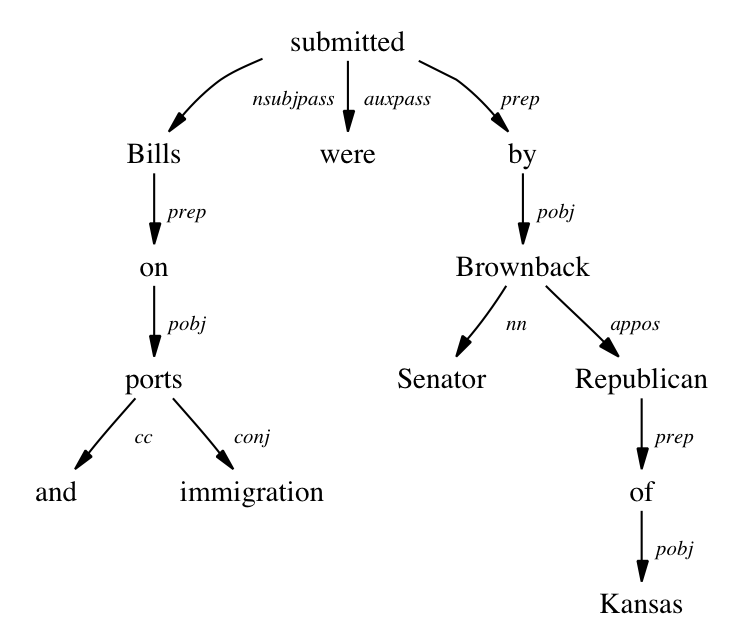
\includegraphics[width=100mm, keepaspectratio]{figures/UD.png}
	\caption{UD graph of "\textit{Bills on ports and immigration were submitted by Senator Brownback, Republican of Kansas.}" Image from \href{https://nlp.stanford.edu/software/stanford-dependencies.shtml}{the Stanford site}}
	\label{fig:UD}
\end{figure}

Universal dependency trees represent the grammatical relationships between the words of a sentence; it gives us the grammatical dependencies between words. They can be easily interpreted with some knowledge of the grammatical structure of languages and they are widely used because of this. UD graphs are highly standardized and are a language independent way to generate the grammatical structure.

One example of a dependency parsed sentence is on Figure~\ref{fig:UD}\footnote{https://nlp.stanford.edu/software/stanford-dependencies.shtml}. You can see the connections and their types between words. Some dependency parsers also predict part-of-speech (POS) tags. For this example sentence the POS tags are the following:
\textbox{Bills: \textit{noun}, on: \textit{preposition}, ports: \textit{noun}, and: \textit{conjunction}, immigration: \textit{noun}, were: \textit{verb}, submitted: \textit{verb}, by: \textit{preposition}, Senator: \textit{noun}, Brownback: \textit{noun}, Republican: \textit{noun}, of: \textit{preposition}, Kansas: \textit{noun}}{}

Dependency trees have been used from the early 20th century based on the work of Lucien Tesni\`ere. In his book titled \textit{\'El\'ements de syntaxe structurale} (Elements of Structural Syntax)\cite{UD} he described the modern grammatical dependency graph structure.

We construct these trees by dependency parsing. There is a multitude of ways we can do that, the library I used in my solution (\href{https://github.com/stanfordnlp/stanfordnlp}{stanfordnlp})\footnote{https://github.com/stanfordnlp/stanfordnlp} utilizes the deep learning based approach.

Most UD parsing methods use treebanks built from parsed corpora, and are used for annotation. Treebanks have been standardized in 2013 by Ryan McDonald's team~\cite{TextRank}. Treebanks are available in multiple languages on the \href{https://universaldependencies.org/}{universal dependency site}.\footnote{\url{https://universaldependencies.org/}} There was a shared task~\cite{ParserSharedTask} to build a parser that is capable of dependency parsing in multiple languages.

%----------------------------------------------------------------------------
\section{Graph format}
%----------------------------------------------------------------------------

The graph\_nets library was developed and published on \href{https://github.com/deepmind/graph_nets}{GitHub}\footnote{\url{https://github.com/deepmind/graph_nets}} by DeepMind in 2018. The team detailed their solutions in the publication titled \textit{Relational inductive biases, deep learning, and graph networks}~\cite{GraphNet}. The graph network was defined to learn graph transformations between relational data. Such relational data can be data from physical systems, sorting problems, shortest path problems.\footnote{\url{https://github.com/deepmind/graph_nets/tree/master/graph_nets/demos}} At first it was not clear whether they can be efficiently trained on real-world data,\footnote{\url{https://github.com/deepmind/graph\_nets/issues/36}} but experiments quickly showed, it can be trained with appropriate relational data.

I defined the extractive summarization as graph transformation, where the input graph is the merged article graph and the output is the said article graph with the nodes and edges that are in the summary graph marked with one and the ones not in the summary graph marked with zero. I used the graph\_nets library to train graph neural networks to learn this graph transformation.
	
The graph\_nets library uses a specific format for graphs, a so called GraphTuple. The user can transform multiple graphs with networkx format or dictionary	 to a GraphTuple object. In my project I used dictionaries because they seemed to be the more straightforward and manageable approach.
The graph dictionary contains the following elements:
\begin{itemize}
	\item nodes: list containing the feature vectors of each node. In my final solution each node's feature vector is the lemma and the part-of-speech tag of the given word 
	\item edges: list containing the feature vectors of each edge. The final feature vector contains the type of each word relation.
	\item globals: global parameter list. I found no relevant use for this parameter in my project.
	\item senders: list containing the indices of the sender nodes in the order of the edges.
	\item receivers: list containing the indices of the receiver nodes in the order of the edges.
\end{itemize}

\begin{figure}[!ht]
	\centering
	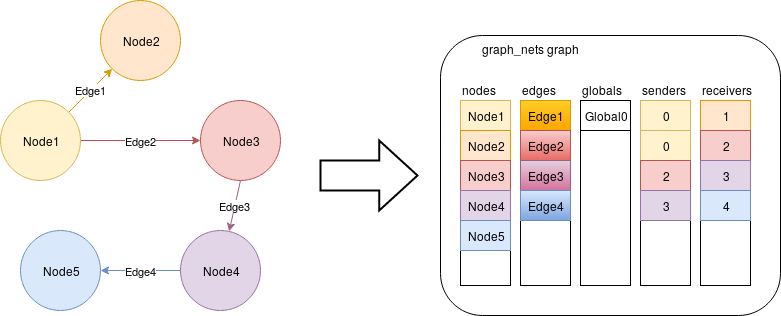
\includegraphics[width=150mm, keepaspectratio]{figures/transform_color.png}
	\caption{Graph transformation to dictionary format.}
	\label{fig:transform_graph}
\end{figure}

On the visual representation Figure \ref{fig:transform_graph} of this kind of graph transformation I highlighted the nodes and edges and the corresponding feature vectors and indices with the same color for easy traceability.
\FloatBarrier

Although I mentioned the transformation between one graph dictionary and one GraphTuple, but one instance of GraphTuple usually contains a batch of multiple graphs. To be able to handle multiple graphs the GraphTuple object has two more fields calculated during the transformation between the list of graph dictionaries and the GraphTuple instance:
\begin{itemize}
	\item n\_node: the number of nodes in each graph.
	\item n\_edge: the number of edges in each graph.
\end{itemize}

\begin{figure}[!ht]
	\centering
	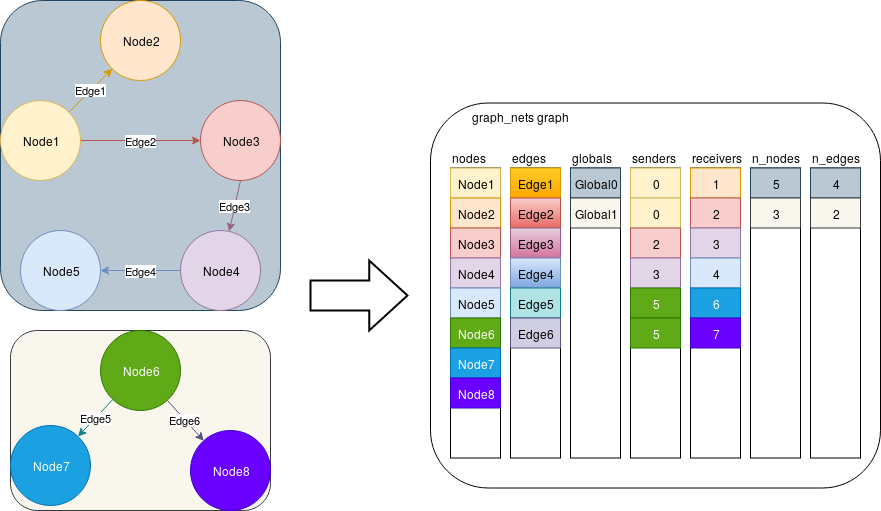
\includegraphics[width=150mm, keepaspectratio]{figures/transform_multiple.png}
	\caption{Graph transformation to GraphTuple format. The dictionary list is not visualized.}
	\label{fig:transform_multiple}
\end{figure}

On the Figure \ref{fig:transform_multiple} depicting this I also applied highlighting on the nodes, edges and graph backgrounds and the corresponding feature vectors and indices with the same color.

\FloatBarrier
%----------------------------------------------------------------------------
\section{Building the graphs}
%----------------------------------------------------------------------------

As I mentioned in the Introduction\ref{sect:Introduction} I used the stanfordnlp library to generate the universal dependency parse trees from the texts. Using the lemma and part of speech (POS) tag of the words I constructed the nodes of the graph the following way: if a word's lemma appears multiple times with the same POS tag in the text I've treated them as one node and the dependencies were merged as edges.

The feature vector a node is the vector of their lemma and POS tag. The feature vector of the edges is the UD relation between the words.

\begin{figure}[!ht]
	\centering
	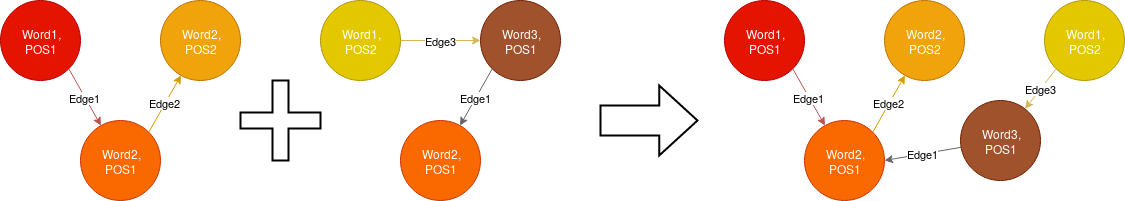
\includegraphics[width=150mm, keepaspectratio]{figures/merge_graphs_color.png}
	\caption{Graph merge.}
	\label{fig:merge_graph_color}
\end{figure}

As you can see at Figure \ref{fig:merge_graph_color}, the resulting graph is not a correct UD graph because the \textit{Word2, POS1} node has multiple incoming edges.

\begin{figure}[!ht]
	\centering
	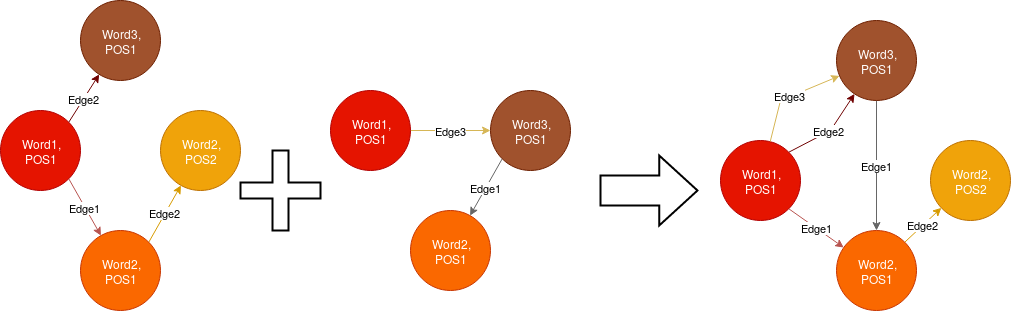
\includegraphics[width=150mm, keepaspectratio]{figures/merge_graphs_color_multiple.png}
	\caption{Graph merge with multiple matching nodes.}
	\label{fig:merge_graph_color_multiple}
\end{figure}

On Figure \ref{fig:merge_graph_color_multiple} you can see how multiple node matches affect the construction of the graph merging.

\begin{figure}[!ht]
	\centering
	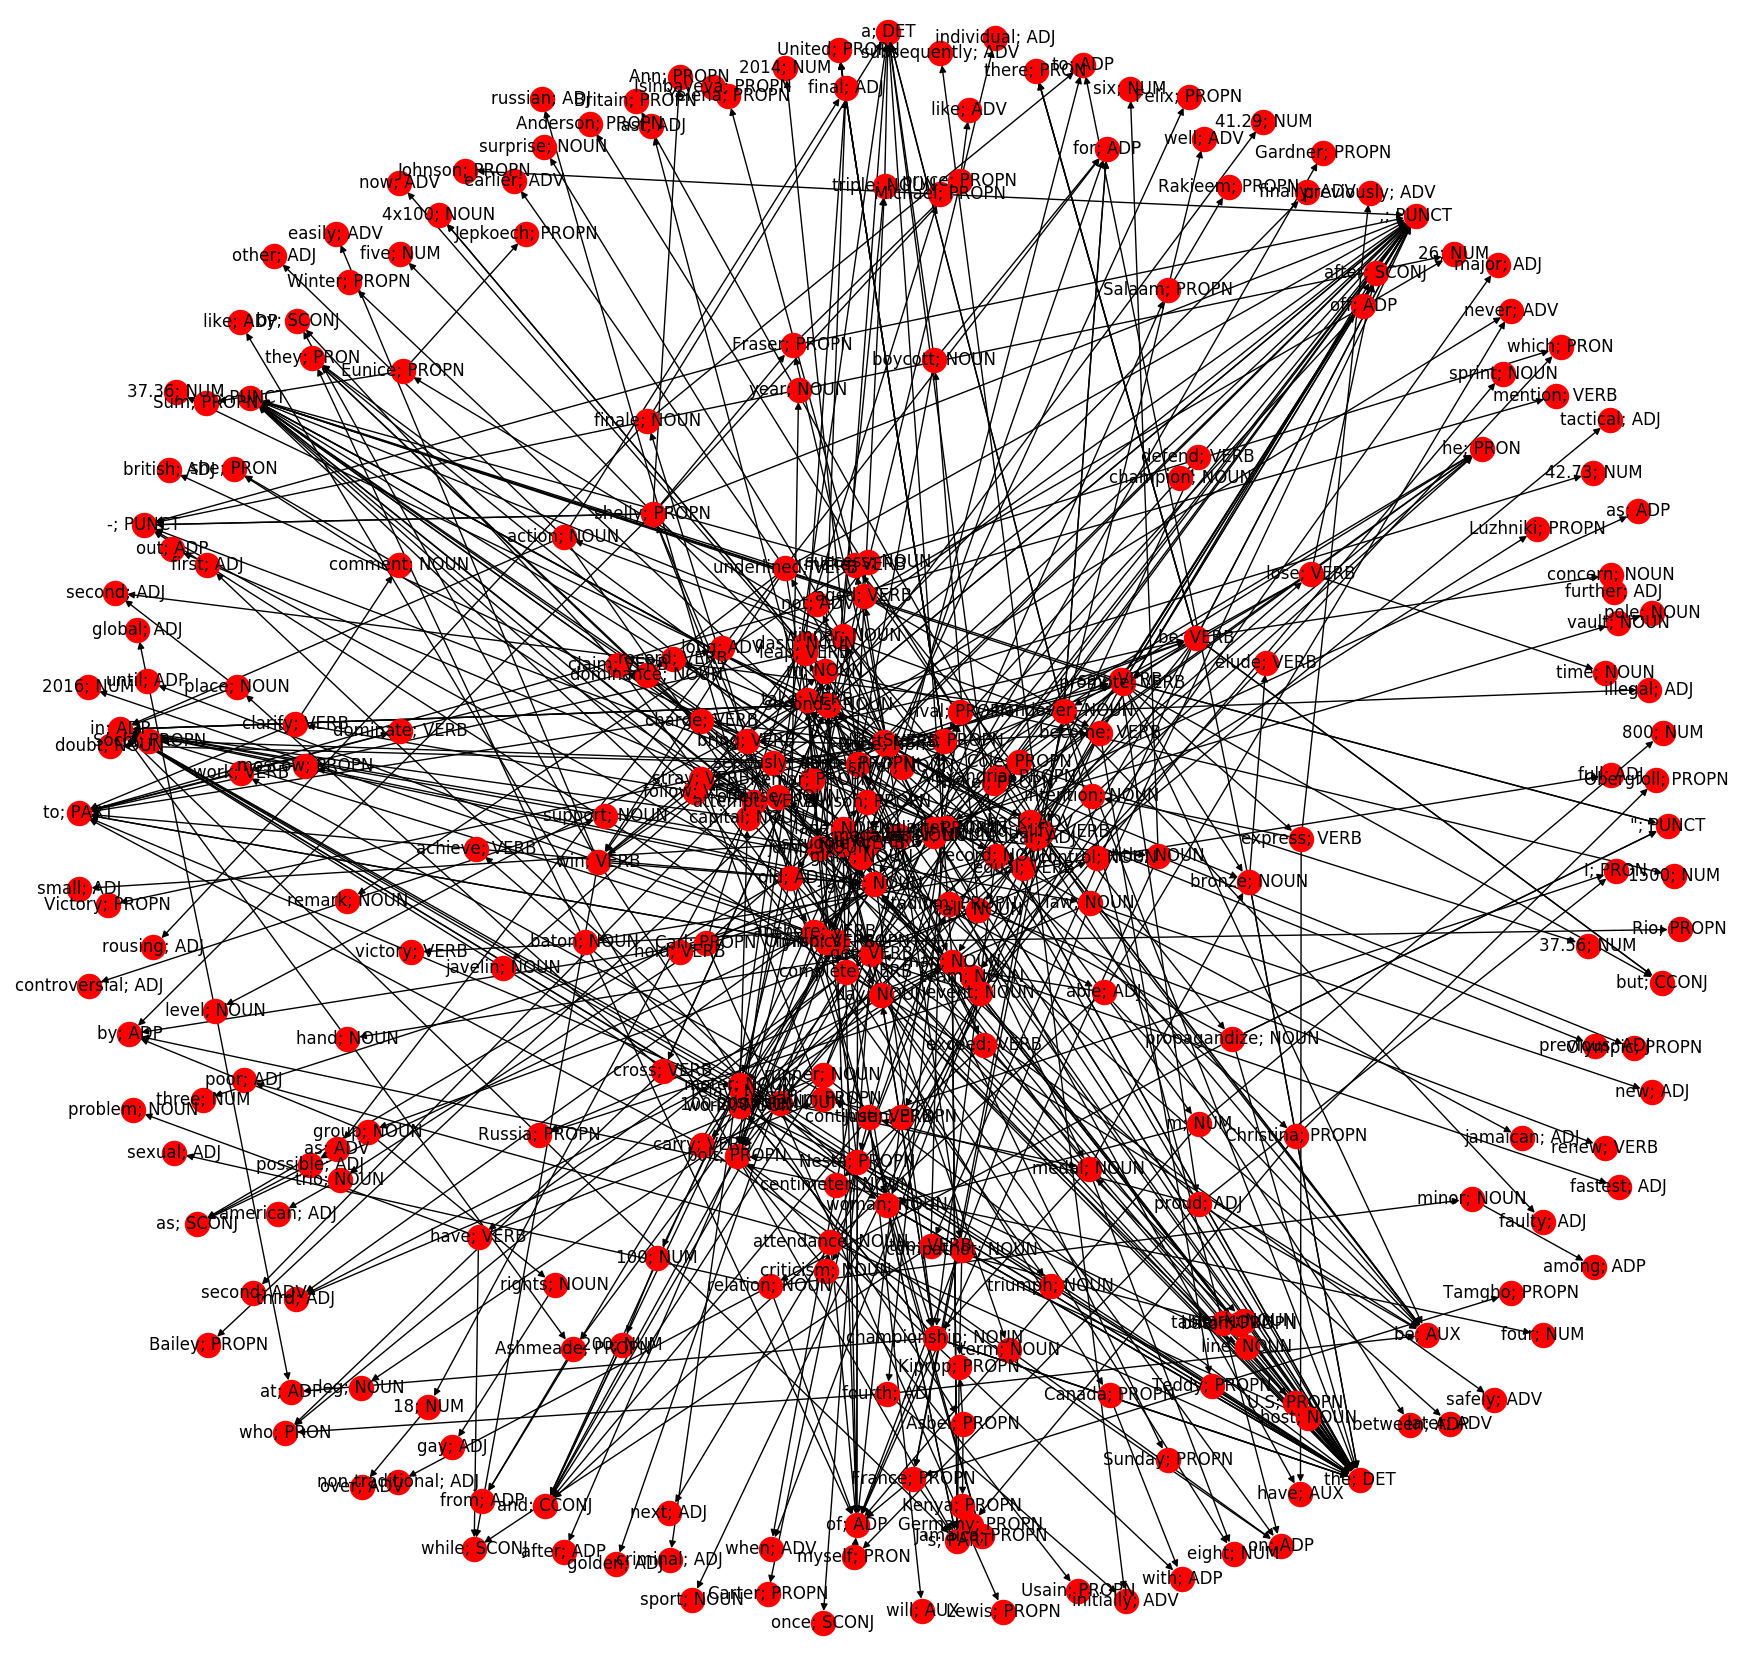
\includegraphics[width=150mm, keepaspectratio]{figures/usain_bolt_article.png}
	\caption{The graph built from the example article.}
	\label{fig:usain_article_graph}
\end{figure}

With this method I was able to represent an article with one large, merged graph, like the one on Figure \ref{fig:usain_article_graph}. As you can see, it is not easily interpretable for a human at first glance, but you can tell, that the nodes with high connectivity appeared frequently. Most of these are stop-words, which I left in the graphs for the connectivity.

\FloatBarrier
%----------------------------------------------------------------------------
\section{Forming the target graphs}
%----------------------------------------------------------------------------
Like I mentioned before, I needed the target graphs to be the same format as the input graph with the summary elements marked. Initially my approach was to try to learn the summaries written by people. For this I needed to generate summary graphs, but their structure was not adequate for training any graph neural network on it. So my solution was the following: I iterated through the edges of the article graph and if the sender node, the receiver node and the edge type matched any edge in the summary I've marked them by adding a 1.0 at the end of their feature vector. Otherwise I appended a 0.0 to the vector.

Similarly I iterated through the nodes as well and checked whether the same feature vector appears in the summary graph and appended 1.0 in case of successful search, 0.0 otherwise.

\begin{figure}[!ht]
	\centering
	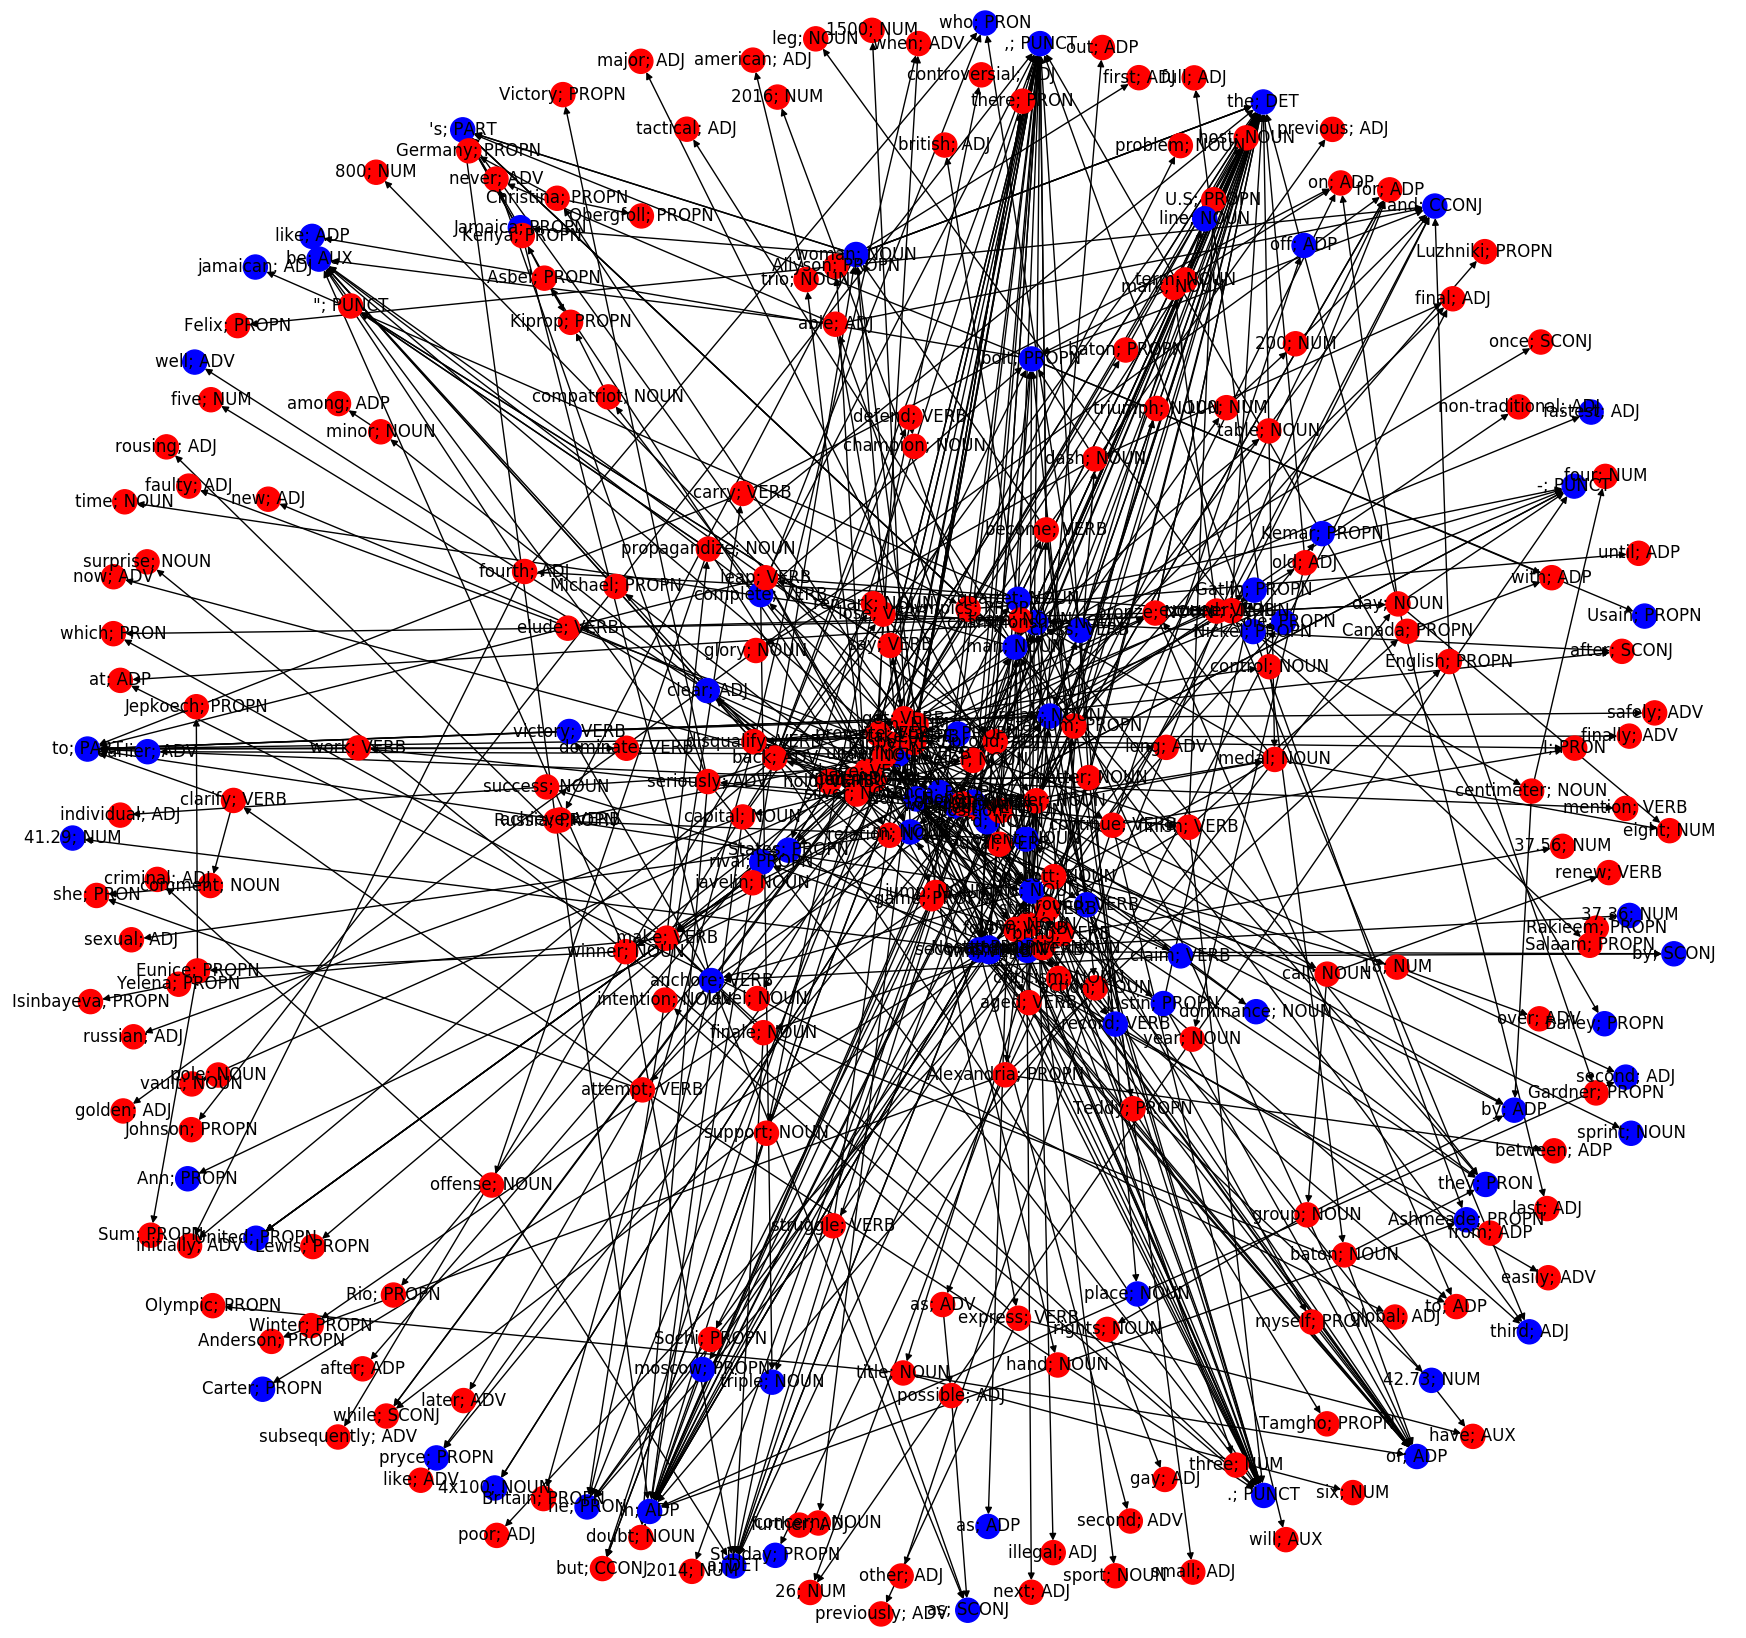
\includegraphics[width=150mm, keepaspectratio]{figures/usain_bolt_colored.png}
	\caption{The colored article graph of the example article. I highlighted the nodes with label 1 with blue.}
	\label{fig:usain_article_graph_colored}
\end{figure}

\begin{figure}[!ht]
	\centering
	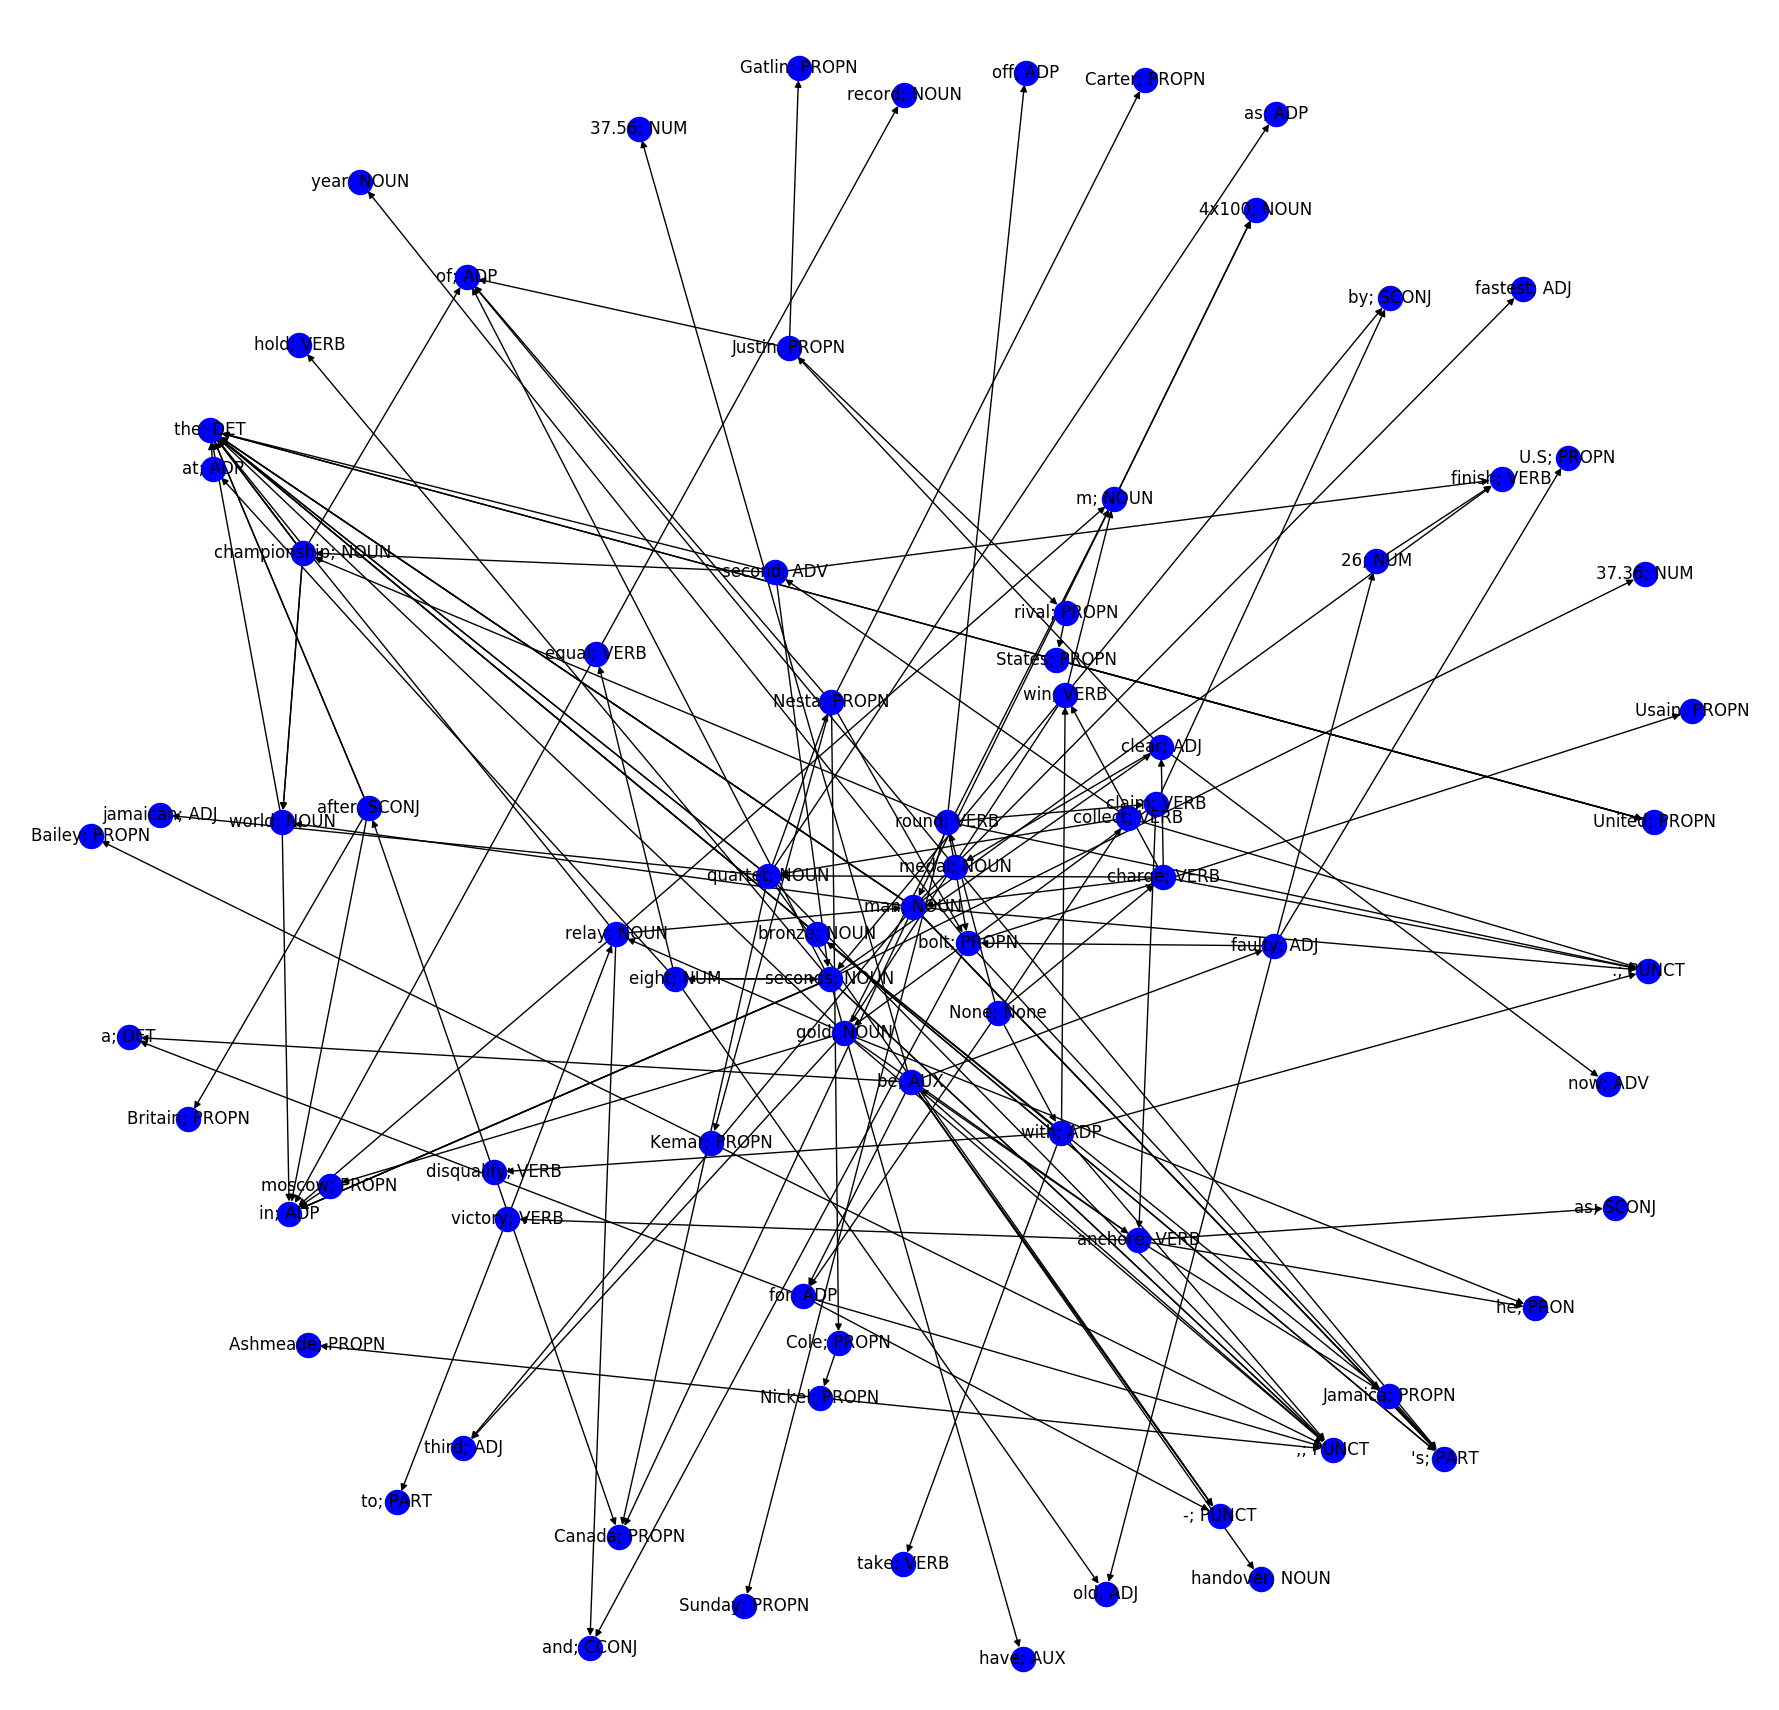
\includegraphics[width=150mm, keepaspectratio]{figures/usain_bolt_summary.png}
	\caption{The summary graph of the example article. This is the subgraph of the article graph with the node labels of 1.}
	\label{fig:usain_summary_graph}
\end{figure}

This way I was able to achieve the same structure, but with marked summary nodes and edges.

The problem with this approach was the fact, that some of the expressions used in the summary did not match up with anything from the original text so the result could not contain the same level of information as the summary graph on it's own.

However, the dataset contained the extracted summaries with the best possible ROUGE score and I decided to use that as the expected output of my neural network. The construction is similar to the previous one, but instead of generating another graph and then trying to find the corresponding parts I only iterated through the UD graphs of the sentences and labeled the nodes and edges in that with the right label.

The graphs resulting from this approach contained more information and proved to be better for training. On Figure \ref{fig:usain_article_graph_colored} and Figure \ref{fig:usain_summary_graph} you can see the results of the first article visualized in two different ways.

%----------------------------------------------------------------------------
\chapter{Graph neural network}\label{sect:GraphNetwork}
%----------------------------------------------------------------------------

\section{Neural Networks}
Artificial neural networks are used for various machine learning and deep learning purposes. In this section I will introduce the basic concepts of artificial neural networks used for supervised learning. Supervised learning is the process of neural network training with a given set of inputs and desired outputs and the goal is to train that system to predict the target outputs with the least error possible.

Most of the contents of this section is from the paper written by \'Ad\'am Kov\'acs and I for the Scientific Students' Associations conference in 2018 \cite{SemParse}.

\subsection{Perceptron}
The perceptron is the building block of the most basic neural networks. It functions as follows: The \(x\) input vector is element-wise multiplied by the \(w\) weight vector and is summed with the \(b\) bias parameter.
\[y = b + \sum_{i=1}^{n} x_i w_i\]

\begin{figure}[!ht]
	\centering
	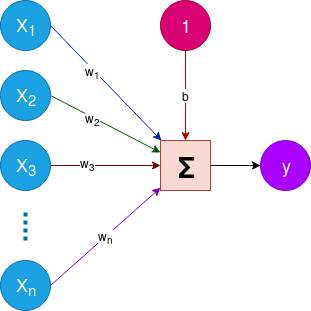
\includegraphics[width=75mm, keepaspectratio]{figures/perceptron.png}
	\caption{A perceptron.}
	\label{fig:perceptron}
\end{figure}

\subsection{Feed forward neural network}

The feed forward or dense neural network is built from perceptrons organized in layers, each layer fully connected to the next layer. The connections each have a weight parameter assigned to them. The nodes are perceptrons with only one slight difference, their output is not necessarily linear.

So called activation functions are used after the summation to bring non-linearity to the model. Such functions are for example the sigmoid, hyperbolic tangent, ReLU functions.

\[\sigma(x) = \frac{1}{1 + e^{-x}}\]
\[tanh(x) = \frac{e^x - e^{-x}}{e^x + e^{-x}}\]
\[relu(x) = \begin{cases}
	x, & \text{if } x > 0\\
	0, & \text{otherwise}
\end{cases}\]

So the result of one neuron in a layer is calculated as follows:

\[\hat{y} = activationFunction(\sum_{i=1}^{m}(x_i * w_i + b))\]

\begin{figure}[!ht]
	\centering
	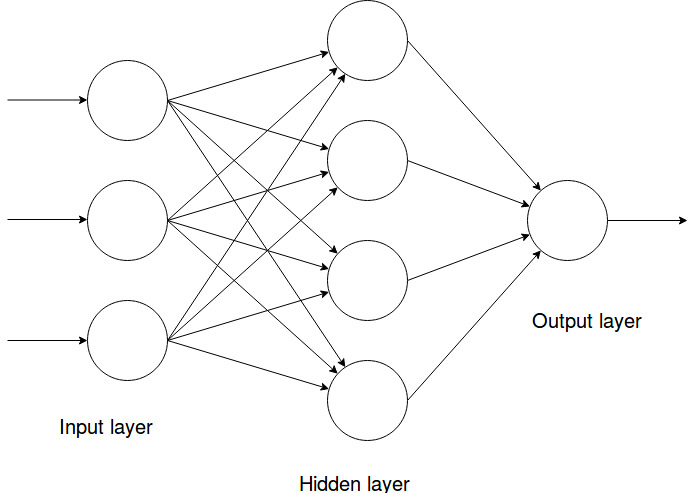
\includegraphics[width=125mm, keepaspectratio]{figures/feed_forward_neural_network.jpg}
	\caption{A feed forward neural network.}
	\label{fig:feed_forward}
\end{figure}

The weight and bias parameters are modified during a process called backpropagation which utilizes the chain rule to propagate the gradient of the loss backwards. The weights and the bias are updated with their difference from the gradient multiplied by a learning rate.

The loss is the difference function between the calculated value and the expected outcome. We don't just calculate the numeric difference in this case, but in case of classification we use the cross entropy function.

\[L = - \sum_{i=1}^{n} y_i \ln(\hat{y_i})\]

The equation above can be used in a multiclass system, where \(n\) is the number of classes and \(\hat{y}\) is the calculated output, while \(y\) is the expected output.

The parameter update happens as follows:

\[\Delta_x L = \sum_{k} \frac{\delta L}{\delta w^k}\frac{\delta w^k}{\delta x}\]

\[w \leftarrow w - \eta \Delta_x L\]

Where \(\eta\) is the learning rate.

The learning rate parameter can also change during the training process. This is called optimization. The main goal of it is to overcome the problems with setting the learning rate (too high can cause us to jump over any good solution, too low results in very slow learning and settling in a local minimum).

One such optimization method is called Adam. It is a cross between two other methods: Adaptive learning rate and Momentum. I used it for the training the models described in the next chapter. The basic idea is slowly degrading the learning rate, based on the previous gradient.

\subsection{Embedding layers}

The function of embedding layers is to turn values to fixed length vectors. They are used mostly in natural language processing to work as word2vec translation. Word2vec is the mechanism to translate a word into vector space.\cite{Word2Vec}

Word embeddings are used in basically all state-of-the art systems related to
natural language processing applications. Mikolov\cite{Mikolov:2013x} showed that word embeddings can be applied for vector operations, like addition or subtraction, and these operations often result in meaningful representation. If we have example words "King", "Man", "Woman", then the vector("King") - vector("Man") + vector("Woman") will most likely result in vector that is close to vector("Queen") in the embedding space. See Figure~\ref{fig:worvec}.

\begin{figure}[!ht]
	\centering
	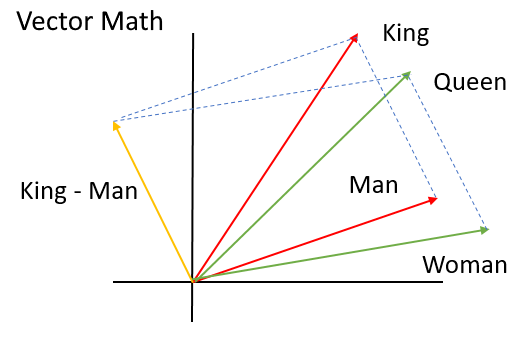
\includegraphics[scale=0.75, keepaspectratio]{figures/vecs.png}
	\caption{An word vector operations.}
	\label{fig:worvec}
\end{figure}

When using embedding layers we want to find vectors for each word so that it can model the word's meaning. We achieve this by looking at the context, the word usually appears in. If two words like \textit{apple} and \textit{orange} usually appear in the same context, than the vectors assigned to these words should have low cosine distance between them.

If you are building an NLP model, the embedding layer should be in the first layer, since its purpose is to make the transition from word to vector, and the word in this case is the input.

\begin{figure}[!ht]
	\centering
	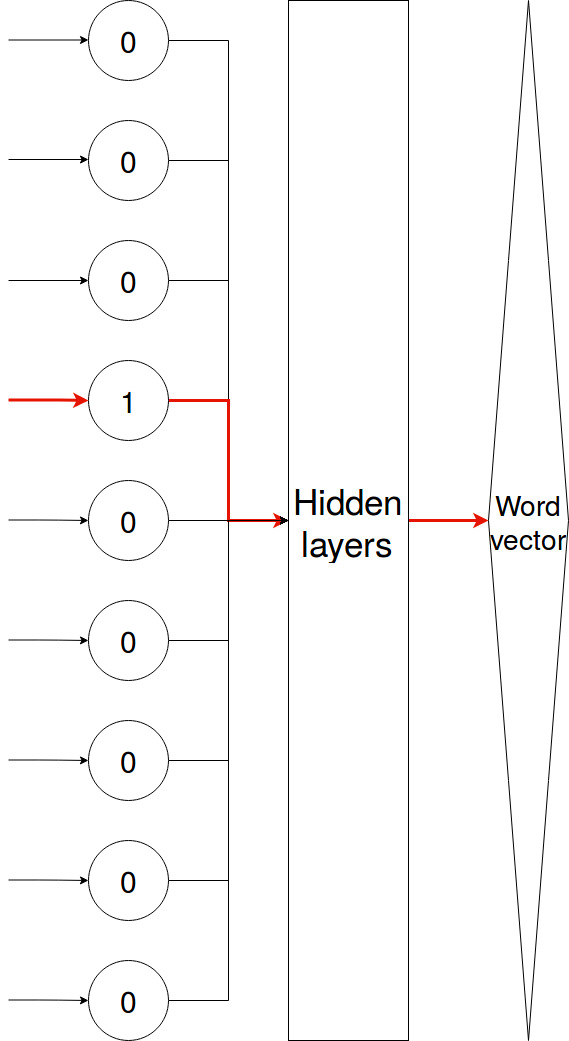
\includegraphics[scale=0.25, keepaspectratio]{figures/embedding_layer.jpg}
	\caption{An embedding layer.}
	\label{fig:embedding_layer}
\end{figure}

The input dimension of this layer is the size of the vocabulary and the output dimension is the size of the dense vector. Usually the vocabulary size greatly exceeds the embedding dimension since the output vectors size is fixed and can range from 300 to 1000, and the vocabulary - depending on the dataset - can be way higher than that. See at Figure~\ref{fig:embedding_layer}.

They work mostly like a lookup table that can be trained. A lot of the times we use pretrained models, like the GloVe embeddings\cite{GloVe} that have been trained on enormous datasets. We can also train them on our specific problem, or use the pretrained and our own embeddings simultaneously.

There has been a huge step forward on this field with the appearance of pre-trained embeddings built from language models. The first such embedding is ELMo \cite{ELMo} which is a deep-contextualized word representation capable to handle character level features as well as the context of a given word.

\subsection{Recurrent Neural Networks}

RNNs~\cite{RNN} can be used in supervised and also unsupervised learning. They are used when the data is sequential, like text, audio, etc.

\begin{figure}[!ht]
	\centering
	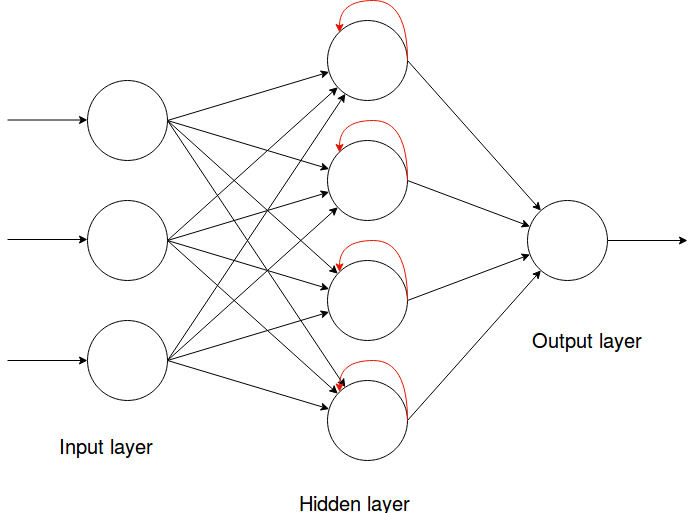
\includegraphics[width=125mm, keepaspectratio]{figures/recurrent_neural_network.jpg}
	\caption{A recurrent neural network.}
	\label{fig:recurrent_net}
\end{figure}

In a simple feed forward neural network, the information only moves in one direction: from the input layer to the output layer. On the other hand recurrent neural networks take into account their immediate past, the output of the network with the previous timestamp. This internal "memory" like functionality allows the network to remember what it had calculated before. This is illustrated at Figure~\ref{fig:recurrent_net}.

At every timestamp the network gets two sets of inputs: the actual input at the timestamp and the hidden state of the network for the previous input. In one iteration it calculates its output using the calculated hidden state in the timestamp. It all could be imagined like the same feed forward network being repeated after one other.

The hidden state mentioned above is the "memory" of the network that is calculated with the previous hidden state and the input.

\begin{figure}[!ht]
	\centering
	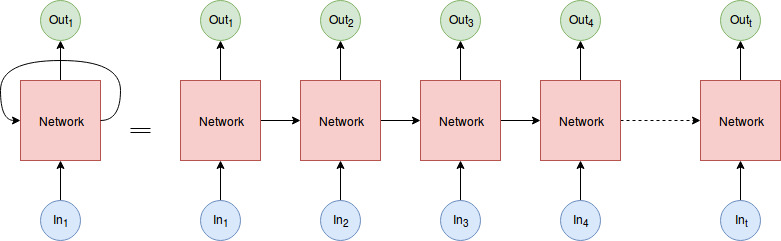
\includegraphics[width=150mm, keepaspectratio]{figures/unrolled.jpg}
	\caption{Unrolled recurrent neural network.}
	\label{fig:unrolled}
\end{figure}

The backpropagation is also slightly different in this case, it's called backpropagation through time, you need to "unroll" the network (see at Figure~\ref{fig:unrolled}), and use the backpropagation starting from the right timestamps. Each timestamp's backpropagation could be understood as backpropagation on a separate feed forward neural network.

The gradient vanishing or explosion can be a problem with this RNN.

There is a multitude of solutions for the exploding gradients, one of which is called gradient clipping. This technique is a very simple yet powerful way of dealing with exploding gradients. All it does is that it limits the size of the gradient, if its norm is higher than a set threshold.

\subsubsection{Long-Short Term Memory}
Long-short term memory networks\cite{LSTM} are the extension of the previously discussed recurrent neural network. The main difference is that it also has an internal long term memory. Usually these type of networks are more reluctant to have the exploding gradient problem.

Like the simple RNN, LSTMs also have hidden states, that are calculated slightly differently.
\\

\begin{minipage}{\textwidth}
	The LSTMs hidden states are calculated using three gates:
	\begin{itemize}
		\item \textbf{input gate}: determines whether to let new input in
		\item \textbf{forget gate}: determines whether to forget an input because it's not relevant anymore
		\item \textbf{output gate}: determines whether to let the input impact the output with the current timestamp
	\end{itemize}
\end{minipage}

These gates are analog and their values ranges from 0 to 1 with the sigmoid function. A simplified depiction can be seen at Figure~\ref{fig:lstm}.
\begin{figure}[!ht]
	\centering
	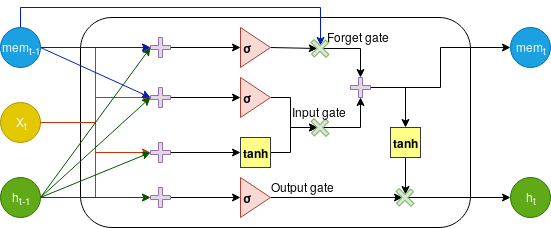
\includegraphics[width=125mm, keepaspectratio]{figures/lstm.png}
	\caption{A long-short term memory network's gates.}
	\label{fig:lstm}
\end{figure}

The sigmoid function allows this structure to be able to learn, meaning that we can use the backpropagation through time method described above.

Long-short term memory networks are used in natural language processing, but also in generative networks, like video or image description generation, text generation and so on.

\subsection{Attention}
The Attention mechanism was first described by Dzmitry Bahdanau in 2015 \cite{Bahdanau:2015} and was used for machine translation. Since then it became a widely used tool in natural language processing. The idea behind this mechanism is that when the neural network predicts the output, it only uses parts of the given input instead of the full input. That is where the most relevant information is concentrated and this mechanism only pays \textit{attention} to these parts and the network has to learn what to pay attention to.

Usually in the "sequence-to-sequence" tasks like machine translation there are two main parts of the model an encoder and a decoder. The encoder and the decoder are usually some type of RNN, mostly LSTM. The encoder is responsible for creating a so called context-vector from the input sequence. This context-vector has a fixed length and it serves as the representation of the sequence inside the model. The decoder then decodes this context-vector to a sequence again, in the case of the machine translation this sequence is in a different language. A depiction can be seen at Figure~\ref{fig:seq_to_seq}.
\begin{figure}[!ht]
	\centering
	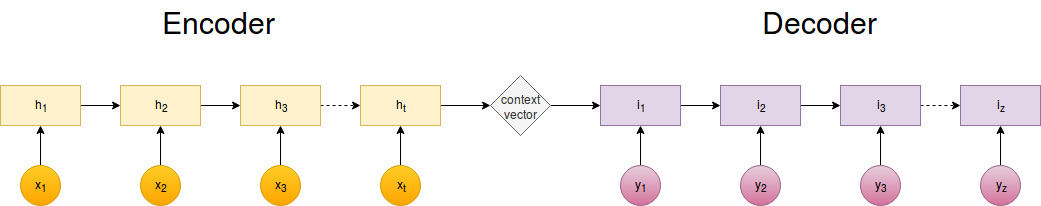
\includegraphics[width=150mm, keepaspectratio]{figures/seq_to_seq.jpg}
	\caption{A sequence-to-sequence model with encoder and decoder.}
	\label{fig:seq_to_seq}
\end{figure}

The attention mechanism was used in the decoder part of this model, the encoder functions the same way. The paper explicitly stated that this attention mechanism relieves the encoder from having to encode every sequence to a fixed length context vector. In this case we have a context vector for every word of the expected output. These context-vectors are the weighted sums of the encoder's states (\textit{annotations}).
\[c_i = \sum_{j=1}^{t} \alpha_ij h_j\]
Where \(\alpha\) parameter is calculated like the following:
\[\alpha_ij = \frac{exp(e_{ij})}{\sum_{k=1}^{t} e_{ik}} \]
and \(e_{ij}\) is its energy
\[e_{ij} = a(s_{i-i}, h_j)\]

\begin{figure}[!ht]
	\centering
	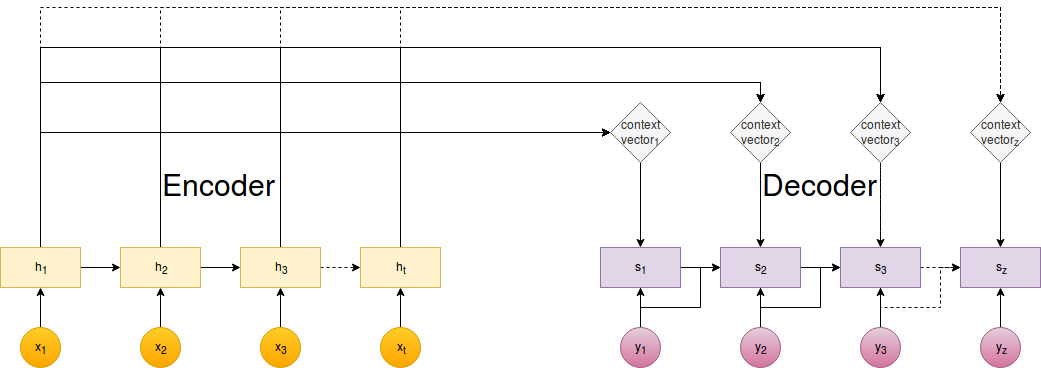
\includegraphics[width=150mm, keepaspectratio]{figures/attention.jpg}
	\caption{A sequence-to-sequence model with encoder-decoder and attention.}
	\label{fig:attention}
\end{figure}

This is an \textit{alignment model} that scores how well the input around \textit{j} and the output around \textit{i} match. This \textit{alignment model} is a feed forward neural network that is trained simultaneously with the other components of the system.
The decoder uses the previous state's output and its assigned context-vector when calculating its own target.
\[s_i = f(s_{i-1}, y_{i-1}, c_i)\]
The attention based model is at Figure~\ref{fig:attention}.


\section{The graph\_nets library}
As I mentioned in the previous chapter graph neural networks are used for graph transformation. Recently an article has been published about the types and possible uses of graph neural networks\cite{SurveyGNN}.  Graph neural networks are used on the field of physics\cite{PhysicsGNN}, computer vision\cite{CVGNN} and also NLP\cite{NLPGNN} but they are still not common.\footnote{\url{https://github.com/thunlp/GNNPapers}}

My main source for understanding the mechanisms of the graph\_nets library was the article titled \textit{Relational inductive biases, deep learning, and graph networks}\cite{GraphNet} and the \href{https://github.com/deepmind/graph_nets/tree/master/graph_nets/demos}{demos} available on GitHub.
The article explains the different approaches of graph transformation learning, most importantly the graph independent model and the graph dependent models.

The most notable difference between the two is the fact that while the graph dependent structure uses the data of the nodes and the edges simultaneously, the graph independent model does train the nodes and edges separately from each other.

Both models can be used under different circumstances, but the can also be used together in training processes.

\subsection{Graph Network block}

The graph\_nets library contains three different block type: EdgeBlock, NodeBlock and GlobalBlock. Each responsible for the propagation of the corresponding tensor through the right function. So we can construct different models for edges, nodes and global parameters.

\textbox{
	\textbf{Definitions from the code}

	The \textit{NodeBlock} updates the features of each node in batch of graphs based on
	the previous node features, the aggregated features of the
	adjacent edges, and the global features of the corresponding graph.
	
	The \textit{EdgeBlock} updates the features of each edge in a batch of graphs based on the previous edge features, the features of the adjacent nodes,
	and the global features of the corresponding graph.
	
	The \textit{GlobalBlock} updates the global features of each graph in a batch based on the previous global features, the aggregated features of the
	edges of the graph, and the aggregated features of the nodes of the graph.
}{}

On top of using these graph structure dependent building blocks the GraphNetwork model (or Graph dependent model for the sake of clarity) it utilizes the updated edge features to calculate the node features and these results are used to update the global features.

\subsection{Graph Independent block}
As the name suggests, in this block every aspect of the graph is independent from another, the defined update functions only take into account their input tensor which can be the node tensor, the edge tensor or the global tensor.

\subsection{Self Attention block}
The graph\_nets library contains a multi-head self attention module which is mostly based on the article titled Attention Is All You Need~\cite{Multihead} which introduced Multi-head attentions.

This mechanism updates the node features based on the node values, node keys and node queries taking into account the structure of the graph.
%----------------------------------------------------------------------------
\chapter{Models}\label{sect:Models}
%----------------------------------------------------------------------------
In this chapter I will introduce the models I experimented with. Encode Process Decode model has been defined in the graph\_nets demos. The SimpleGraphAttention and the GraphAttention models are defined by me.

\section{Encode Process Decode model}
This model has been tested and used in the demos provided on \href{https://github.com/deepmind/graph_nets/blob/master/graph_nets/demos/models.py}{GitHub}\footnote{\url{https://github.com/deepmind/graph_nets/blob/master/graph_nets/demos/models.py}}.
\begin{figure}[!ht]
	\centering
	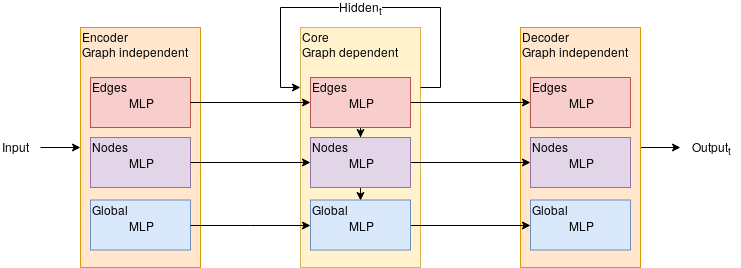
\includegraphics[width=150mm, keepaspectratio]{figures/EPD.png}
	\caption{Representation of the model.}
	\label{fig:encode-process-decode}
\end{figure}

As it is shown on the Figure~\ref{fig:encode-process-decode} above the model consist of 3 different parts.

\subsection{Encoder}
The encoder model is a graph independent model that uses multi layer perceptrons and layer normalization on the global attributes, the edge feature vectors and the node feature vectors. There are no shared variables between the multi layer perceptrons.

\subsection{Core}
This is the only graph dependent part of the model. It also uses multi layer perceptrons and layer normalization as the previous one, but the graph dependency enables it to use the predicted edge features to influence the node features and these impact the global feature.

This section of the network is repeated resulting in a hidden state that gets feed forward again in the Core section. Each step has its own output with its timestamp.

\subsection{Decoder}
The decoder model has the same structure as the encoder. It does not use any kind of activation on the last layer, which enables it to better generalize, but also making it harder to use on a specific project eq. classifying whether or not the summary graph contains the given node or edge.

\section{SimpleGraphAttention model}
I based the architecture of this model on the Encode Process Decode model. I modified it to be better suited for NLP problems, because it transforms the input words into higher dimension vector space, as you can see on Figure~\ref{fig:graph-attention0}.

\begin{figure}[!ht]
	\centering
	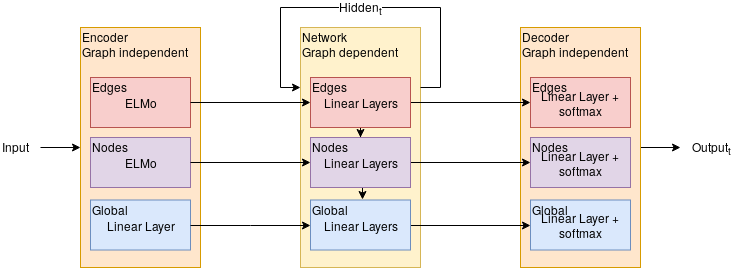
\includegraphics[width=150mm, keepaspectratio]{figures/GA0.png}
	\caption{Representation of the model.}
	\label{fig:graph-attention0}
\end{figure}

\subsection{Encoder}

The encoder part of the network contains two Embedding layers; one for the lemmas of the nodes and one for the edges' type (See Figure~\ref{fig:graph-attention0-encoder}). 

\begin{figure}[!ht]
	\centering
	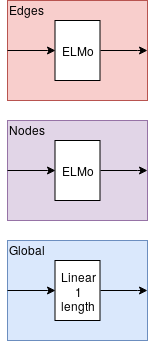
\includegraphics[scale=0.5]{figures/GA0_encoder.png}
	\caption{Representation of the encoder part of the model.}
	\label{fig:graph-attention0-encoder}
\end{figure}

The second one's necessity is questionable, since it does not contain as much information and could be also represented with a simple one-hot encoded vector, since it has not as high dimensionality as the nodes. However I decided I leave it in the model and make it a changeable parameter of the network.

For the global features I only used a simple linear layer without activation functions, since it does not need to be encoded in any way. All of these blocks work independently from each other, updating their respective blocks, because the parts are defined as the edge, node and global functions for a GraphIndependent block.

\subsection{Network}

The Network, or core part of the model consists of activated linear layers with differing sizes as depicted on Figure~\ref{fig:graph-attention0-network}.

\begin{figure}[!ht]
	\centering
	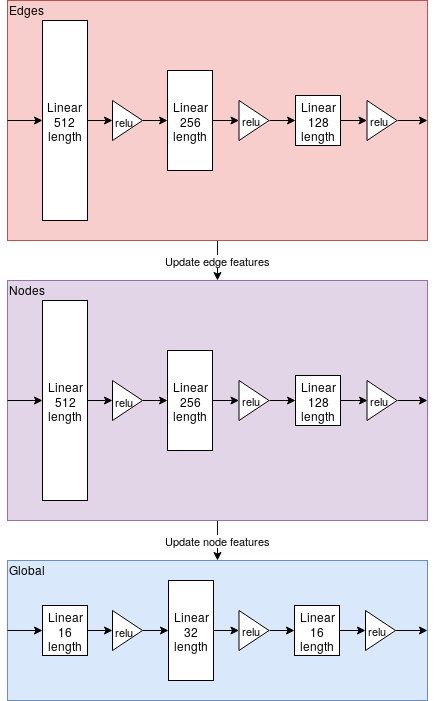
\includegraphics[scale=0.5]{figures/GA0_network.png}
	\caption{Representation of the network part of the model.}
	\label{fig:graph-attention0-network}
\end{figure}

Since this section of the model is graph dependent, after each feature update, the next block gets the updated feature vectors instead of the original ones.

\subsection{Decoder}

The decoder part of the model is also graph independent just like the encoder and it simply serves the function of the softmax output of the whole network. Its structure is presented on Figure~\ref{fig:graph-attention0-decoder}.

\begin{figure}[!ht]
	\centering
	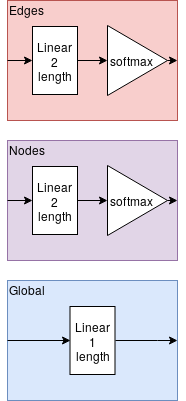
\includegraphics[scale=0.5]{figures/GA0_decoder.png}
	\caption{Representation of the decoder part of the model.}
	\label{fig:graph-attention0-decoder}
\end{figure}

\section{GraphAttention model}
The starting point of this model was the \textit{SimpleGraphAttention} model which I further developed using recent advancements regarding attention in graphs. There was two versions of this model, one that used LSTM cells in the Network part in the node block, and the other that used only linear layers. Since the main structure is the same I only included the graphical presentation on Figure~\ref{fig:graph-attention1} and Figure~\ref{fig:graph-attention1-network} of the later version. This one proved to be more usable due to the large amount of memory usage of the LSTM cells.

\begin{figure}[!ht]
	\centering
	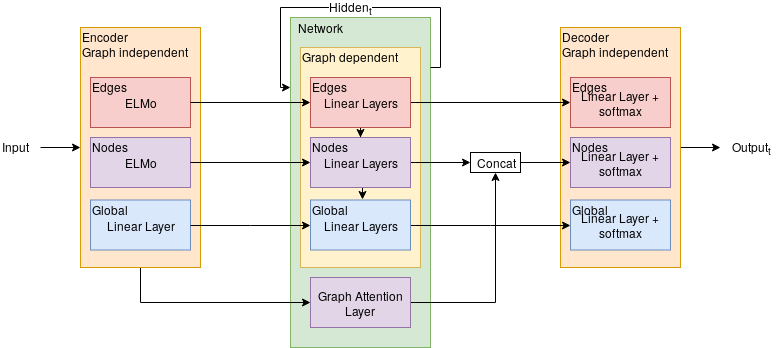
\includegraphics[width=150mm, keepaspectratio]{figures/GA1.png}
	\caption{Representation of the model.}
	\label{fig:graph-attention1}
\end{figure}


The Encoder and Decoder segments of the network are identical to their correspondences in the SimpleGraphAttention model.

\subsection{Network and Graph Attentional Layer}
The network part of the model went under some changes compared to the SimpleGraphAttention model's Network. The most notable change is the new, independent part of the network, called GAT. You can see a simplification of the network on Figure~\ref{fig:graph-attention1-network}.

\begin{figure}[!ht]
	\centering
	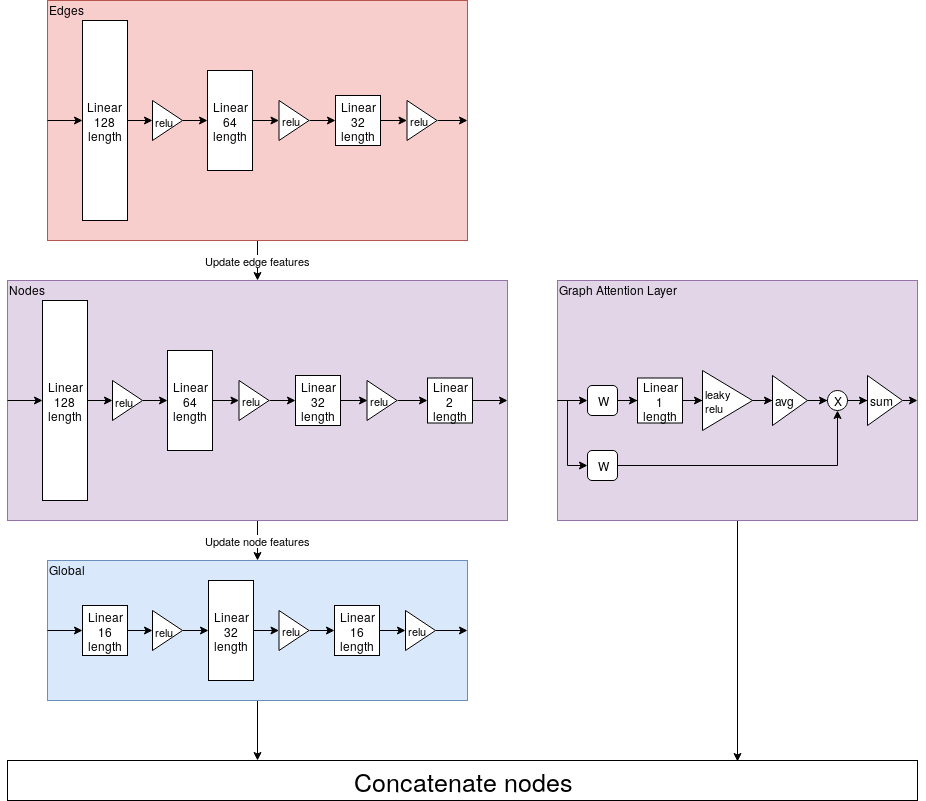
\includegraphics[scale=0.5]{figures/GA1_network.png}
	\caption{Representation of the network part of the model.}
	\label{fig:graph-attention1-network}
\end{figure}

The Graph Attentional Layer has been described in a 2018 paper titled \textit{Graph Attention Networks}~\cite{GAT}. It was designed to work well with Graph Convolutional Network structures, but I was able to implement it for the Graph Neural Network architecture as well.

This layer updates node features the following way: Suppose the features of the nodes are \(h_i\), we define a weight matrix \(W \in \mathbb{R}^{input\ features} \times \mathbb{R}^{output\ features} \) and a feed forward attention layer.

Let the normalized attention coefficients be:

\[a_{ij} =  \frac{exp(LeakyReLU(attention(W\vec{h_i} || W\vec{h_j})))}{\sum_{k \in i\ neighbors} exp(LeakyReLU(attention(W\vec{h_i} || W\vec{h_k})))}\]
if i and j are neighbors.

\[\vec{h_i}' = \sigma(\sum_{j \in i\ neighbours}a_{ij}W\vec{h_j})\]

Since we are working with multi-head attention, the update equation is modified as follows:
\[\vec{h_i}' = \sigma(\frac{1}{K} \sum_{k=1}^{K}\sum_{j \in i\ neighbours}a_{ij}^kW^k\vec{h_j})\]

Where K is the number of heads in the multi-head attention.

%----------------------------------------------------------------------------
\chapter{Experiments and results}\label{sect:Experiments}
%----------------------------------------------------------------------------
\section{Evaluation methods}

I used three methods to evaluate the results. The most basic method is the accuracy measure, which calculates the ratio of the correct answers as follows:

\[accuracy = \frac{correct\ answer}{all\ answer}\]

Since we are talking about graphs we need to measure the accuracy on the nodes and (if we are also training on them) the edges.
\[accuracy_{nodes\ and\ edges} = \frac{correct\ nodes + correct\ edges}{all\ nodes + all\ edges}\]

The other general evaluation metric in case of classification is the F-score. This is better for evaluating the results of a classification because it is not so greatly affected by the distribution of the classes. For this we need to calculate the true positive, true negative, false positive and false negative measures for every class. See on Figue~\ref{fig:TP_TN_FP_FN}.

\begin{figure}[!ht]
	\centering
	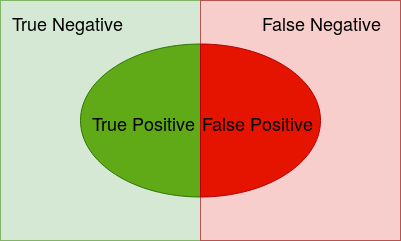
\includegraphics[width=100mm, keepaspectratio]{figures/F_score.png}
	\caption{The visual representation of the concept of true positive, true negative, false positive and false negative measures.}
	\label{fig:TP_TN_FP_FN}
\end{figure}


\[TP_{node==0} = number\ of\ correctly\ guessed\ node==0\]
\[TN_{node==0} = number\ of\ correctly\ guessed\ node!=0\]
\[FP_{node==0} = number\ of\ incorrectly\ guessed\ node==0\]
\[FN_{node==0} = number\ of\ incorrectly\ guessed\ node!=0\]

With these measures we can calculate the precision and recall. The precision tells us the ratio of correct guesses of the class out of every time the model predicted that class. The recall is the ratio of the correct guesses out of every instance that are actually in the class. The harmonic mean of the precision and recall is the F-score.

\[precision = \frac{TP}{TP + FN}\]
\[recall = \frac{TP}{TP + FP}\]

\[F1 = 2 * \frac{precision * recall}{precision + recall}\]

I constructed extractive summaries from the resulting graphs and the original articles multiple ways described in section~\ref{ssect:ExperimnetsAndResults} and calculated the various ROUGE scores for each method's output.

\section{Experiments and results}\label{ssect:ExperimnetsAndResults}
I have experimented with both the Encode Process Decode and the Graph Attention Network models with varying success.
\subsection{Encode Process Decode}
At first I tried to get the Encode-Process-Decode model to predict whether to put something in the summary graph or not using only the word ids as features, but realized it would probably be more sufficient to also use the POS tags.

I also experimented with different loss functions, but for now i decided to use softmax cross entropy with output feature sizes of 2.

Training on more, than 7000 articles for 5 epochs (Early stopping stopped it from running any longer). I've got the following results.
\begin{table}[!h]
	\centering
	\begin{tabular}{| c | c |}
		\hline
		Test loss & 0.447 \\ \hline
		Test accuracy over nodes and edges & 0.958 \\ \hline
	\end{tabular}
	\caption{Softmax cross entropy loss and accuracy on the test set}
\end{table}

\begin{table}[!h]
	\centering
	\begin{tabular}{| c | c | c | c |}
		\hline
		 & precision & recall & f1 \\ \hline \hline
		edges labeled 0&0.96&1.0&0.98  \\ \hline
		edges labeled 1 & 0.0 & 0.0 & 0.0 \\ \hline
		nodes labeled 0 & 0.915 & 0.985 & 0.949 \\ \hline
		nodes labeled 1 & 0.628 & 0.213 & 0.319 \\ \hline
	\end{tabular}
	\caption{The classification report on the test set. Nodes and edges labeled 1 are the ones that were in the summary.}
\end{table}

As it is clear from this the network hardly ever classifies a node as "1", meaning that is should be in the summary graph, but when it does it is 62.8\% accurate.

This model has not been further evaluated.

\subsection{SimpleGraphAttention Network}
I trained the network on the whole training set (80\% of the whole dataset) for 3 epochs. It stopped after the third epoch because of the early stopping mechanism.

I evaluated the trained network on the test set and the results are the following:

\begin{table}[!h]
	\centering
	\begin{tabular}{| c | c |}
		\hline
		Test loss & 0.809 \\ \hline
		Test accuracy over nodes and edges& 0.724 \\ \hline
	\end{tabular}
	\caption{Softmax cross entropy loss and accuracy on the test set}
\end{table}

\begin{table}[!h]
	\centering
	\begin{tabular}{| c | c | c | c |}
		\hline
		& precision & recall & f1 \\ \hline \hline
		nodes labeled 0 & 0.819 & 0.814 & 0.816 \\ \hline
		nodes labeled 1 & 0.534 & 0.542 & 0.538 \\ \hline
	\end{tabular}
	\caption{The classification report on the test set. Nodes and edges labeled 1 are the ones that were in the summary.}
\end{table}

\subsubsection{Summary reconstruction and evaluation}
I tried three different approaches at the summary extraction, each have been evaluated by the ROUGE scoring mechanism. For this I used the perl based pyrouge package.

\paragraph{Reconstruction with the node average}

This reconstruction method scores each sentence of the original article using the equation below where the \(score_{word}\) is the predicted probability of the word (node) being in the summary graph.

\[score_{sentence} = \frac{\sum_{word \in sentence\ and\ word \notin stopwords} score_{word}}{|word \in sentence\ and\ word \notin stopwords|}\]

Based on the calculated score of each sentence we can order them by their relevance and keep the four most relevant sentence from the article as the summary.

This method does not utilize the information of the graph structure nor does it prefer longer sentences.

\begin{longtable}{| l | l | l | l | l |}
	\hline
	\textbf{Evaluation method}&\textbf{Metric}&\textbf{System}&\textbf{Gensim}&\textbf{Extracted}\\ \hline \hline		
	\multirow{3}{*}{\textbf{ROUGE-1}}
		&Average Recall&0.39057&0.56350&0.73912 \\
		&Average Precision&0.23650&0.20366&0.33846 \\ 
		&Average F1&0.27641&0.28692&0.44619 \\ \hline \hline
	\multirow{3}{*}{\textbf{ROUGE-2}}
		&Average Recall&0.12562&0.20801&0.39292 \\
		&Average Precision&0.07189&0.07546&0.18290 \\
		&Average F1&0.08597&0.10587&0.23900 \\ \hline \hline
	\multirow{3}{*}{\textbf{ROUGE-3}}
		&Average Recall&0.06508&0.11009&0.246448 \\
		&Average Precision&0.03694&0.04068&0.11801 \\
		&Average F1&0.04424&0.05656&0.15226 \\ \hline \hline
	\multirow{3}{*}{\textbf{ROUGE-4}}
		&Average Recall&0.04171&0.07074&0.17230 \\
		&Average Precision&0.02395&0.02666&0.08483 \\
		&Average F1&0.02846&0.03671&0.10807 \\ \hline \hline
	\multirow{3}{*}{\textbf{ROUGE-L}}
		&Average Recall&0.24031&0.34467&0.51007 \\
		&Average Precision&0.14231&0.12093&0.23272 \\
		&Average F1&0.16713&0.17149&0.30654 \\ \hline \hline
	\multirow{3}{*}{\textbf{ROUGE-W-1.2}}
		&Average Recall&0.09211&0.12907&0.19517 \\
		&Average Precision&0.11261&0.09360&0.18583 \\
		&Average F1&0.09242&0.10068&0.17739 \\ \hline \hline
	\multirow{3}{*}{\textbf{ROUGE-S*}}
		&Average Recall&0.14421&0.27925&.48162 \\
		&Average Precision&0.05248&0.04148&0.11587 \\
		&Average F1&0.06344&0.06513&0.16621 \\ \hline \hline
	\multirow{3}{*}{\textbf{ROUGE-SU*}}
		&Average Recall&0.15604&0.29271&0.49149 \\
		&Average Precision&0.05775&0.04401&0.12013 \\
		&Average F1&0.06957&0.06914&0.17242 \\ \hline
	\caption{ROUGE scores on the test set with reconstruction method using only the node scores}
\end{longtable}

\paragraph{Reconstruction with just the graph structure}

Contrary to the previous version this construction method does not use the output of the graph neural network but it is included here as contrast and as a step toward the next summarization method.

\begin{eqnarray*}
	score_{sentence} = \sum_{edge \in sentence\ graph} &[1\ if\ sender\ word \notin stopwords] + \\&[1\ if\ receiver\ word \notin stopwords]
\end{eqnarray*}

The ordering is based on this score. The summary contains the four best sentences.

\begin{longtable}{| l | l | l | l | l |}
	\hline
	\textbf{Evaluation method}&\textbf{Metric}&\textbf{System}&\textbf{Gensim}&\textbf{Extracted}\\ \hline \hline
	\multirow{3}{*}{\textbf{ROUGE-1}}
		&Average Recall&0.54166&0.56350&0.73912 \\
		&Average Precision&0.18856&0.20366&0.33846 \\ 
		&Average F1&0.26990&0.28692&0.44619 \\ \hline \hline
	\multirow{3}{*}{\textbf{ROUGE-2}}
		&Average Recall&0.18824&0.20801&0.39292 \\
		&Average Precision&0.06688&0.07546&0.18290 \\
		&Average F1&0.09491&0.10587&0.23900 \\ \hline \hline
	\multirow{3}{*}{\textbf{ROUGE-3}}
		&Average Recall&0.09844&0.11009&0.246448 \\
		&Average Precision&0.03593&0.04068&0.11801 \\
		&Average F1&0.05042&0.05656&0.15226 \\ \hline \hline
	\multirow{3}{*}{\textbf{ROUGE-4}}
		&Average Recall&0.06315&0.07074&0.17230 \\
		&Average Precision&0.02365&0.02666&0.08483 \\
		&Average F1&0.03282&0.03671&0.10807 \\ \hline \hline
	\multirow{3}{*}{\textbf{ROUGE-L}}
		&Average Recall&0.32680&0.34467&0.51007 \\
		&Average Precision&0.11053&0.12093&0.23272 \\
		&Average F1&0.15918&0.17149&0.30654 \\ \hline \hline
	\multirow{3}{*}{\textbf{ROUGE-W-1.2}}
		&Average Recall&0.12214&0.12907&0.19517 \\
		&Average Precision&0.08543&0.09360&0.18583 \\
		&Average F1&0.09396&0.10068&0.17739 \\ \hline \hline
	\multirow{3}{*}{\textbf{ROUGE-S*}}
		&Average Recall&0.25325&0.27925&.48162 \\
		&Average Precision&0.03534&0.04148&0.11587 \\
		&Average F1&0.05684&0.06513&0.16621 \\ \hline \hline
	\multirow{3}{*}{\textbf{ROUGE-SU*}}
		&Average Recall&0.26694&0.29271&0.49149 \\
		&Average Precision&0.03758&0.04401&0.12013 \\
		&Average F1&0.06048&0.06914&0.17242 \\ \hline
	\caption{ROUGE scores on the test set with reconstruction method using just the graph structure}
\end{longtable}

\paragraph{Reconstruction with the graph structure and the node scores}

This method is the blend of the previous two. It utilizes the structure of the graph but also uses the output of the graph neural network.
\begin{eqnarray*}
	score_{sentence} = \sum_{edge \in sentence\ graph} &[score_{sender\ word}\ if\ sender\ word \notin stopwords] + \\&[score_{receiver\ word}\ if\ receiver\ word \notin stopwords]
\end{eqnarray*}
\begin{longtable}{| l | l | l | l | l |}
	\hline
	\textbf{Evaluation method}&\textbf{Metric}&\textbf{System}&\textbf{Gensim}&\textbf{Extracted}\\ \hline \hline
	\multirow{3}{*}{\textbf{ROUGE-1}}
		&Average Recall&0.56795&0.56350&0.73912 \\
		&Average Precision&0.21344&0.20366&0.33846 \\ 
		&Average F1&0.29885&0.28692&0.44619 \\ \hline \hline
	\multirow{3}{*}{\textbf{ROUGE-2}}
		&Average Recall&0.21968&0.20801&0.39292 \\
		&Average Precision&0.08345&0.07546&0.18290 \\
		&Average F1&0.11608&0.10587&0.23900 \\ \hline \hline
	\multirow{3}{*}{\textbf{ROUGE-3}}
		&Average Recall&0.11917&0.11009&0.246448 \\
		&Average Precision&0.04626&0.04068&0.11801 \\
		&Average F1&0.06368&0.05656&0.15226 \\ \hline \hline
	\multirow{3}{*}{\textbf{ROUGE-4}}
		&Average Recall&0.07688&0.07074&0.17230 \\
		&Average Precision&0.03053&0.02666&0.08483 \\
		&Average F1&0.03282&0.04157&0.10807 \\ \hline \hline
	\multirow{3}{*}{\textbf{ROUGE-L}}
		&Average Recall&0.34952&0.34467&0.51007 \\
		&Average Precision&0.12771&0.12093&0.23272 \\
		&Average F1&0.17993&0.17149&0.30654 \\ \hline \hline
	\multirow{3}{*}{\textbf{ROUGE-W-1.2}}
		&Average Recall&0.13174&0.12907&0.19517 \\
		&Average Precision&0.09944&0.09360&0.18583 \\
		&Average F1&0.10571&0.10068&0.17739 \\ \hline \hline
	\multirow{3}{*}{\textbf{ROUGE-S*}}
		&Average Recall&0.28093&0.27925&.48162 \\
		&Average Precision&0.04521&0.04148&0.11587 \\
		&Average F1&0.07070&0.06513&0.16621 \\ \hline \hline
	\multirow{3}{*}{\textbf{ROUGE-SU*}}
		&Average Recall&0.29450&0.29271&0.49149 \\
		&Average Precision&0.04788&0.04401&0.12013 \\
		&Average F1&0.07492&0.06914&0.17242 \\ \hline
	\caption{ROUGE scores on the test set with reconstruction method using both graph structure and the node scores}
\end{longtable}

\subsubsection{Example}
To better visualize the results I compare the summary graph from Chapter~\ref{sect:DataProcessing} (Figure~\ref{fig:usain_summary_graph} and) to the calculated graph (Figure~\ref{fig:usain_bolt_predicted0}). The generated summaries are also written below.

\begin{figure}[!ht]
	\centering
	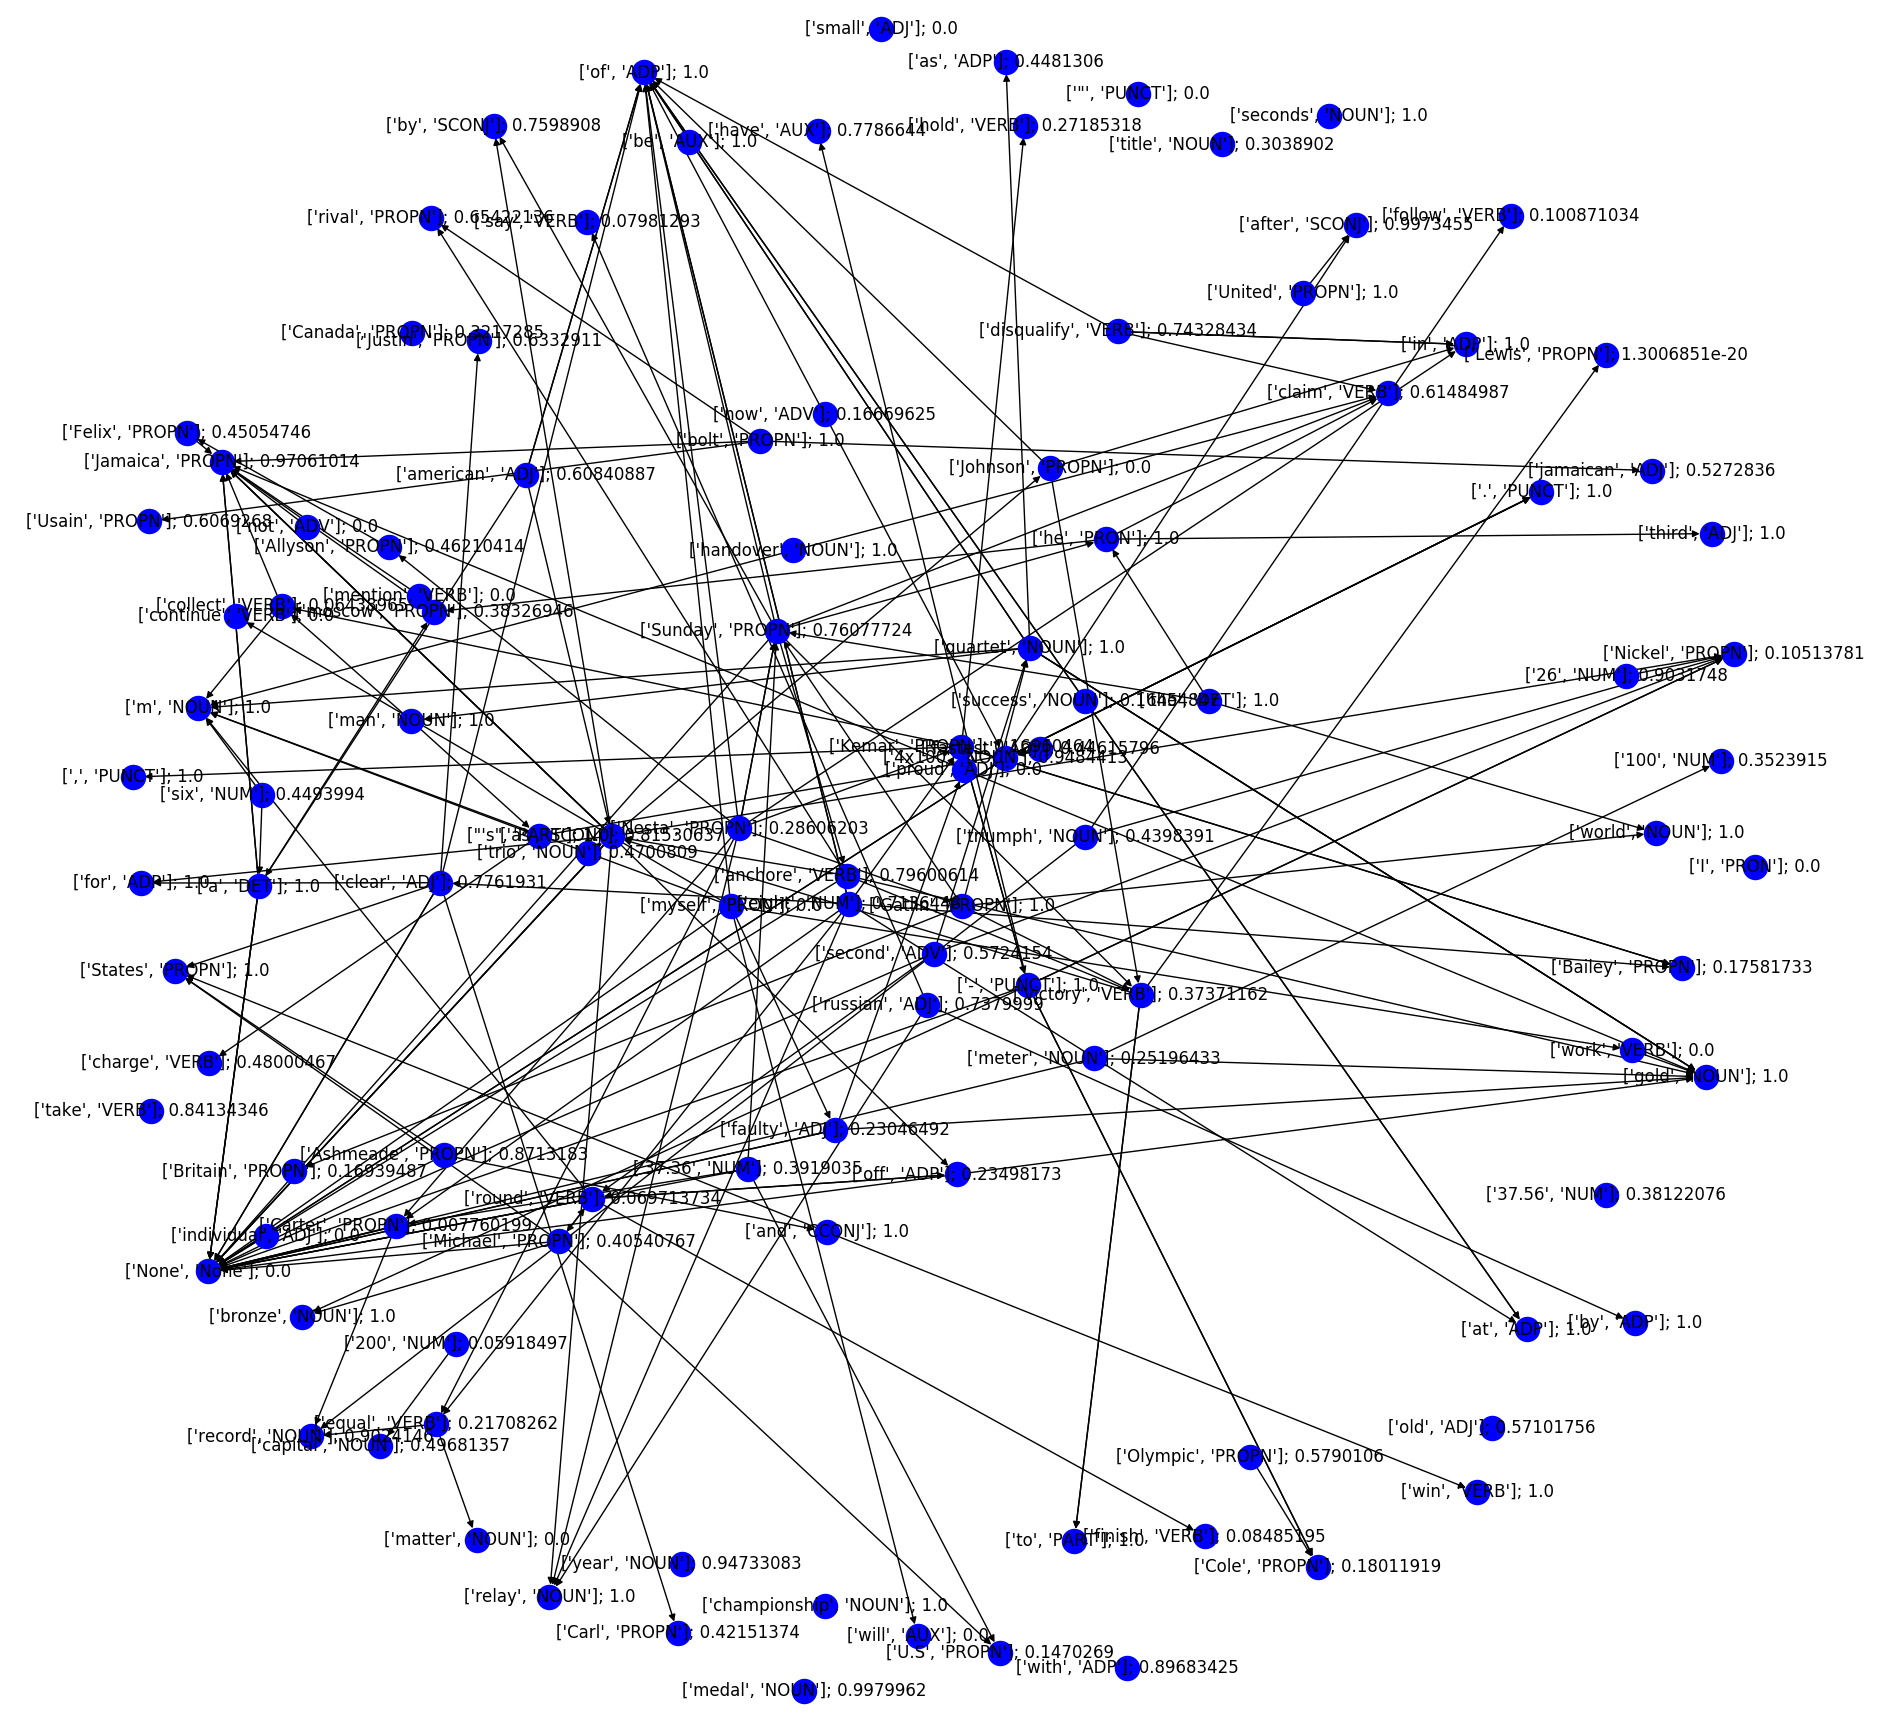
\includegraphics[width=150mm, keepaspectratio]{figures/usain_bolt_predicted.png}
	\caption{The calculated summary graph of the example article with just the nodes labeled 1.}
	\label{fig:usain_bolt_predicted0}
\end{figure}

\textbox{
	\textbf{Reconstruction with the node average}
	
	Fraser-Pryce, like Bolt aged 26, became the first woman to achieve three golds in the 100-200 and the relay.
	Usain Bolt rounded off the world championships Sunday by claiming his third gold in Moscow as he anchored Jamaica to victory in the men's 4x100m relay.
	The British quartet, who were initially fourth, were promoted to the bronze which eluded their men's team.
	Bolt's final dash for golden glory brought the eight-day championship to a rousing finale, but while the hosts topped the medal table from the United States there was criticism of the poor attendances in the Luzhniki Stadium.
	
	\textbf{Reconstruction with just the graph structure}
	
	The 26-year-old Bolt has now collected eight gold medals at world championships, equaling the record held by American trio Carl Lewis, Michael Johnson and Allyson Felix, not to mention the small matter of six Olympic titles.
	Earlier, Jamaica's women underlined their dominance in the sprint events by winning the 4x100m relay gold, anchored by Shelly-Ann Fraser-Pryce, who like Bolt was completing a triple.
	The fastest man in the world charged clear of United States rival Justin Gatlin as the Jamaican quartet of Nesta Carter, Kemar Bailey-Cole, Nickel Ashmeade and Bolt won in 37.36 seconds.
	Defending champions, the United States, were initially back in the bronze medal position after losing time on the second handover between Alexandria Anderson and English Gardner, but promoted to silver when France were subsequently disqualified for an illegal handover.
	
	\textbf{Reconstruction with the graph structure and the node scores}
	
	The fastest man in the world charged clear of United States rival Justin Gatlin as the Jamaican quartet of Nesta Carter, Kemar Bailey-Cole, Nickel Ashmeade and Bolt won in 37.36 seconds.
	Defending champions, the United States, were initially back in the bronze medal position after losing time on the second handover between Alexandria Anderson and English Gardner, but promoted to silver when France were subsequently disqualified for an illegal handover.
	Germany's Christina Obergfoll finally took gold at global level in the women's javelin after five previous silvers, while Kenya's Asbel Kiprop easily won a tactical men's 1500m final.
	Earlier, Jamaica's women underlined their dominance in the sprint events by winning the 4x100m relay gold, anchored by Shelly-Ann Fraser-Pryce, who like Bolt was completing a triple.}{
	\caption{Example article summaries}}

\subsection{GraphAttention Network}

I trained this model on ten-thousand data for 3 epochs. In each epoch the network trained on different data, all in all I used thirty-thousand input and target output. It stopped after the third epoch because of the early stopping mechanism.

Due to time constraints I was unable to train the network on the whole training data.

I evaluated the trained network and the results are the following:

\begin{table}[!h]
	\centering
	\begin{tabular}{| c | c |}
		\hline
		Test loss & 0.7996 \\ \hline
		Test accuracy over nodes and edges& 0.685 \\ \hline
	\end{tabular}
	\caption{Softmax cross entropy loss and accuracy on the test set}
\end{table}

\begin{table}[!h]
	\centering
	\begin{tabular}{| c | c | c | c |}
		\hline
		& precision & recall & f1 \\ \hline \hline
		nodes labeled 0 & 0.851 & 0.711 & 0.775 \\ \hline
		nodes labeled 1 & 0.431 & 0.638 & 0.514 \\ \hline
	\end{tabular}
	\caption{The classification report on the test set. Nodes and edges labeled 1 are the ones that were in the summary.}
\end{table}

\subsubsection{Summary reconstruction and evaluation}
I tried the same reconstruction method for the results of the GraphAttention model. Keep in mind that this model has been trained for less time and on less data.

\paragraph{Reconstruction with the graph structure and the node scores}

\begin{longtable}{| l | l | l | l | l |}
	\hline
	\textbf{Evaluation method}&\textbf{Metric}&\textbf{System}&\textbf{Gensim}&\textbf{Extracted}\\ \hline \hline
	\multirow{3}{*}{\textbf{ROUGE-1}}
	&Average Recall&0.56020&0.56350&0.73912 \\
	&Average Precision&0.20580&0.20366&0.33846 \\ 
	&Average F1&0.29006&0.28692&0.44619 \\ \hline \hline
	\multirow{3}{*}{\textbf{ROUGE-2}}
	&Average Recall&0.21028&0.20801&0.39292 \\
	&Average Precision&0.07823&0.07546&0.18290 \\
	&Average F1&0.10951&0.10587&0.23900 \\ \hline \hline
	\multirow{3}{*}{\textbf{ROUGE-3}}
	&Average Recall&0.11300&0.11009&0.246448 \\
	&Average Precision&0.04297&0.04068&0.11801 \\
	&Average F1&0.05954&0.05656&0.15226 \\ \hline \hline
	\multirow{3}{*}{\textbf{ROUGE-4}}
	&Average Recall&0.07278&0.07074&0.17230 \\
	&Average Precision&0.02831&0.02666&0.08483 \\
	&Average F1&0.03881&0.04157&0.10807 \\ \hline \hline
	\multirow{3}{*}{\textbf{ROUGE-L}}
	&Average Recall&0.34276&0.34467&0.51007 \\
	&Average Precision&0.12238&0.12093&0.23272 \\
	&Average F1&0.17356&0.17149&0.30654 \\ \hline \hline
	\multirow{3}{*}{\textbf{ROUGE-W-1.2}}
	&Average Recall&0.12889&0.12907&0.19517 \\
	&Average Precision&0.09510&0.09360&0.18583 \\
	&Average F1&0.10214&0.10068&0.17739 \\ \hline \hline
	\multirow{3}{*}{\textbf{ROUGE-S*}}
	&Average Recall&0.27247&0.27925&.48162 \\
	&Average Precision&0.04199&0.04148&0.11587 \\
	&Average F1&0.07070&0.06623&0.16621 \\ \hline \hline
	\multirow{3}{*}{\textbf{ROUGE-SU*}}
	&Average Recall&0.28611&0.29271&0.49149 \\
	&Average Precision&0.04453&0.04401&0.12013 \\
	&Average F1&0.07028&0.06914&0.17242 \\ \hline
	\caption{ROUGE scores on the test set with reconstruction method using both graph structure and the node scores}
\end{longtable}

\subsubsection{Example}
Similarly to the previous case I compared the summary graph from Chapter~\ref{sect:DataProcessing} (Figure~\ref{fig:usain_summary_graph} and) to the calculated graph (Figure~\ref{fig:usain_bolt_predicted1}). The generated summaries are also written below.

\begin{figure}[!ht]
	\centering
	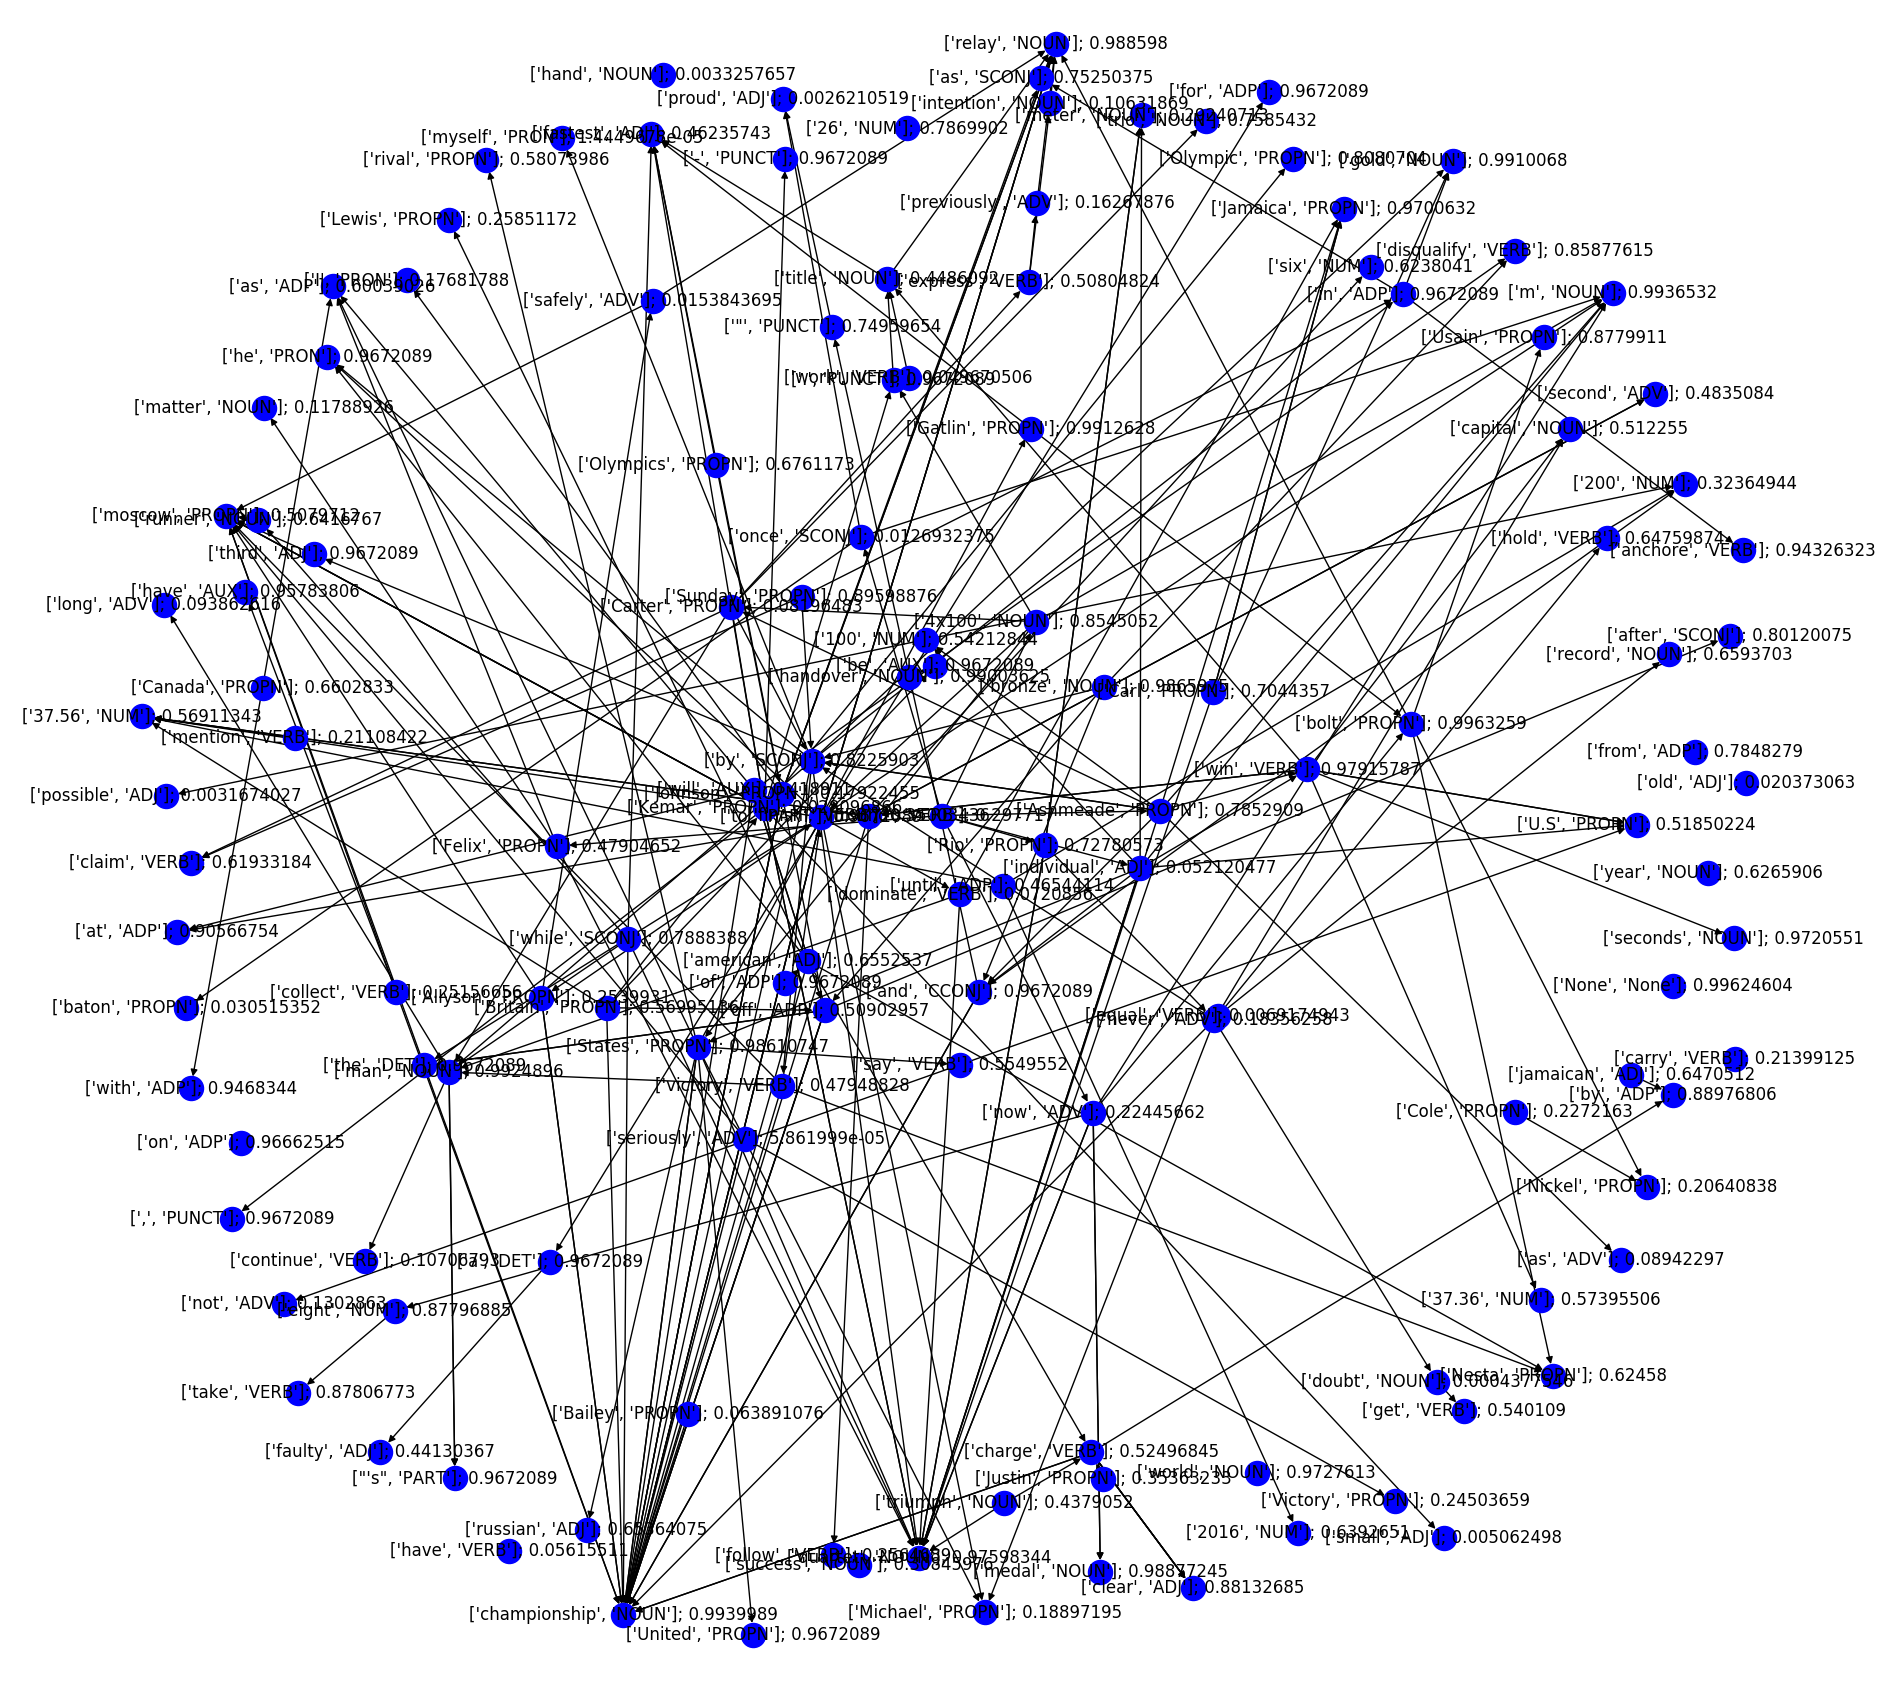
\includegraphics[width=150mm, keepaspectratio]{figures/usain_bolt_predicted_attended.png}
	\caption{The calculated summary graph of the example article with just the nodes labeled 1.}
	\label{fig:usain_bolt_predicted1}
\end{figure}

\textbox{
	\textbf{Reconstruction with the node average}
	
	Usain Bolt rounded off the world championships Sunday by claiming his third gold in Moscow as he anchored Jamaica to victory in the men's 4x100m relay.
	Fraser-Pryce, like Bolt aged 26, became the first woman to achieve three golds in the 100-200 and the relay.
	The British quartet, who were initially fourth, were promoted to the bronze which eluded their men's team.
	The U.S finished second in 37.56 seconds with Canada taking the bronze after Britain were disqualified for a faulty handover.
	
	\textbf{Reconstruction with just the graph structure}
	
	The 26-year-old Bolt has now collected eight gold medals at world championships, equaling the record held by American trio Carl Lewis, Michael Johnson and Allyson Felix, not to mention the small matter of six Olympic titles.
	Earlier, Jamaica's women underlined their dominance in the sprint events by winning the 4x100m relay gold, anchored by Shelly-Ann Fraser-Pryce, who like Bolt was completing a triple.
	The fastest man in the world charged clear of United States rival Justin Gatlin as the Jamaican quartet of Nesta Carter, Kemar Bailey-Cole, Nickel Ashmeade and Bolt won in 37.36 seconds.
	Defending champions, the United States, were initially back in the bronze medal position after losing time on the second handover between Alexandria Anderson and English Gardner, but promoted to silver when France were subsequently disqualified for an illegal handover.
	
	\textbf{Reconstruction with the graph structure and the node scores}
	
	The fastest man in the world charged clear of United States rival Justin Gatlin as the Jamaican quartet of Nesta Carter, Kemar Bailey-Cole, Nickel Ashmeade and Bolt won in 37.36 seconds.
	Defending champions, the United States, were initially back in the bronze medal position after losing time on the second handover between Alexandria Anderson and English Gardner, but promoted to silver when France were subsequently disqualified for an illegal handover.
	Earlier, Jamaica's women underlined their dominance in the sprint events by winning the 4x100m relay gold, anchored by Shelly-Ann Fraser-Pryce, who like Bolt was completing a triple.
	Germany's Christina Obergfoll finally took gold at global level in the women's javelin after five previous silvers, while Kenya's Asbel Kiprop easily won a tactical men's 1500m final.}{}
%----------------------------------------------------------------------------
\chapter{Conclusion and future work}\label{sect:Future}
%----------------------------------------------------------------------------
In my opinion we only started to explore the possibilities of this technique in the realms of natural language processing research and there are still a lot of open questions. The results show that the SimpleGraphAttention model trained on the extracted summaries can achieve within the confidence range of the benchmark gensim TextRank based algorithm's ROUGE score.

My plans for the future include further experimenting with the optimization, modifying the graph attention, and trying out new summary reconstruction methods and new structures.

Modifications of the graph attention layer may include taking into account the edge types in some way because the current one only accounts for the node connectivity. I might reintroduce a modified edge loss for the training process but experiments are needed to determine whether it would be beneficial for the network, since previous iterations suggested otherwise.

In conclusion I think there is room for further development and this research area is highly promising. I would like to delve into graph neural networks even more now that I've come to know them better.
%----------------------------------------------------------------------------
\chapter*{Acknowledgement}\addcontentsline{toc}{chapter}{Acknowledgement}
%----------------------------------------------------------------------------

I would like to express my gratitude to my consultant, \emph{\vikkonzulens} and \emph{Recski G�bor} who helped me tremendously with this project.

I would also like to thank my boyfriend, \emph{Roland Szab�}, family and friends who were absolutely supportive during this time.

%\listoffigures\addcontentsline{toc}{chapter}{�br�k jegyz�ke}
%\listoftables\addcontentsline{toc}{chapter}{T�bl�zatok jegyz�ke}

\bibliography{mybib}
\addcontentsline{toc}{chapter}{Bibliography}
\bibliographystyle{plain}

%----------------------------------------------------------------------------
\appendix
%----------------------------------------------------------------------------
\chapter*{Appendices}\addcontentsline{toc}{chapter}{Appendices}\label{sect:Appendices}
\setcounter{chapter}{1}  % a fofejezet-szamlalo az angol ABC 1. betuje (A) lesz
\newcommand{\tab}[1]{\hspace{.1\textwidth}\rlap{#1}}


%----------------------------------------------------------------------------
\section{Modules and packages}
%----------------------------------------------------------------------------
\begin{figure}[!ht]
	\centering
	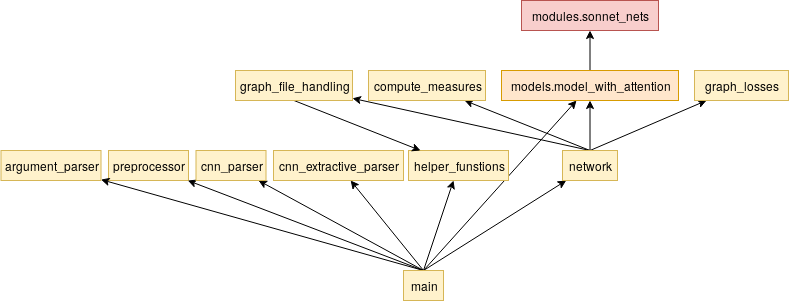
\includegraphics[width=150mm, keepaspectratio]{figures/packages_GraphTransformations.png}
	\caption{The most important modules and packages in the project}
	\label{fig:packages}
\end{figure}

\subsection{Functions and classes in each relevant module}

\begin{itemize}
	\item main.py
	\begin{itemize}
		\item predict function
		\item preprocess function
		\item test function
		\item train function
		\item visualize function
	\end{itemize}
	\item preprocessor.py
	\begin{itemize}
		\item dependency\_parse function
		\item process\_line function
		\item main function
	\end{itemize}
	\item cnn\_parser.py
	\begin{itemize}
		\item highlight\_to\_sentences function
		\item graph\_builder function
		\item main function
	\end{itemize}
	\item cnn\_extractive\_parser.py
	\begin{itemize}
		\item feature\_appender function
		\item article\_graph\_builder function
		\item main function
	\end{itemize}
	\item helper\_functions.py
	\begin{itemize}
		\item is\_valid\_graph function
		\item print\_graphs\_tuple function
		\item visualize\_graph function
		\item visualize\_original\_graph function
		\item visualize\_graph\_with\_colors function
	\end{itemize}
	\item network.py
	\begin{itemize}
		\item generate\_placeholder function
		\item train\_model function
		\item run\_session function
		\item train\_generator function
		\item predict function
		\item predict\_one\_graph function
		\item test function
	\end{itemize}
	\item compute\_measures.py
	\begin{itemize}
		\item compute\_accuracy function
		\item compute\_accuracy\_on\_nodes function
		\item compute\_accuracy\_ratio function
		\item compute\_one\_tp\_tn\_fp\_fn function
		\item compute\_tp\_tn\_fp\_fn function
		\item add\_tp\_tn\_fp\_fn function
		\item compute\_precision\_recall\_f1 function
	\end{itemize}
	\item graph\_losses.py
	\begin{itemize}
		\item regression\_loss function
		\item binary\_categorical\_loss function
		\item softmax\_loss function
		\item softmax\_loss\_on\_nodes function
	\end{itemize}
	\item graph\_file\_handling.py
	\begin{itemize}
		\item process\_line function
		\item load\_graphs function
		\item generate\_graph function
		\item get\_first\_batch\_graph\_dict function
		\item save\_predicted\_graphs function
	\end{itemize}
	\item models.model\_with\_attention.py
	\begin{itemize}
		\item Encoder class
		\item SimpleGraphAttention class
		\item GraphAttention class
	\end{itemize}
	\item modules.sonnet\_nets.py
	\begin{itemize}
		\item ActivatedLSTM class
		\item ActivatedLinear class
		\item NodeEmbedding class
		\item EdgeEmbedding class
		\item SimplifiedSelfAttention class
		\item GraphAttentionLayer class
	\end{itemize}
\end{itemize}

%----------------------------------------------------------------------------
\section{Class diagram}
%----------------------------------------------------------------------------
\begin{figure}[!ht]
	\centering
	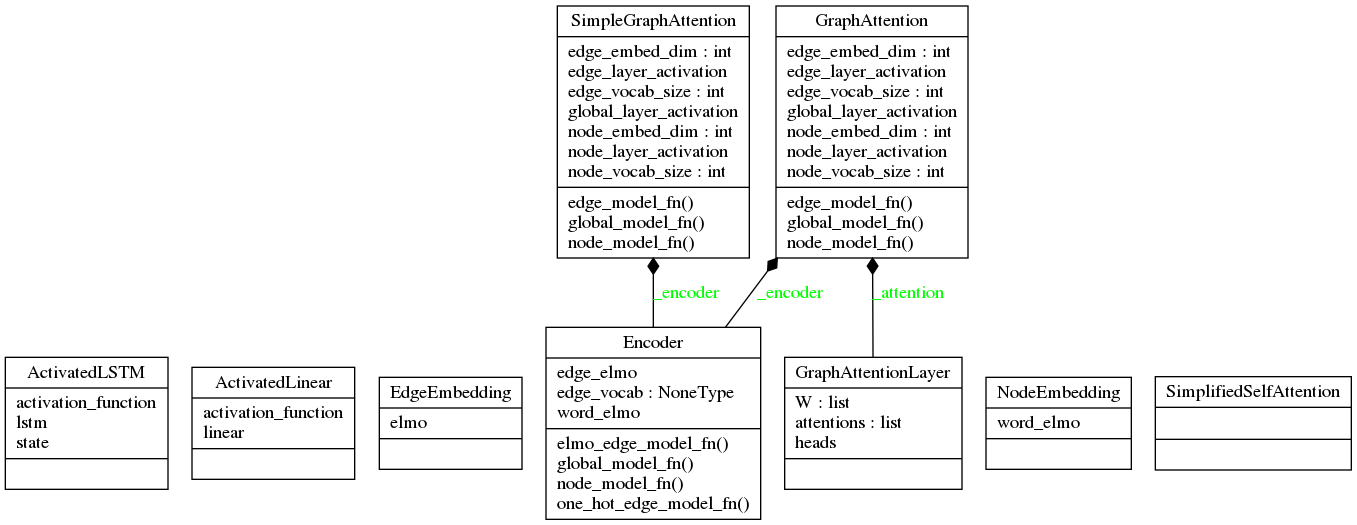
\includegraphics[width=150mm, keepaspectratio]{figures/classes_GraphTransformations.png}
	\caption{The classes in the project. The image was generated using \href{https://www.logilab.org/blogentry/6883}{Pyreverse}}
	\label{fig:classes}
\end{figure}




\label{page:last}
\end{document}
